\chapter{Post-Flight Analysis} \label{postflight}

\section{Overview}
This chapter discusses the post flight analysis of the thermal-mechanical model. In the first section, an overall summary of the flight campaign in Timmins, Ontario is presented, including work done while in Timmins and the overall results of the flight. The next section describes the mechanical results of the flight, in terms of how the mechanical design fared and some fixes that need to be made. The rest of the chapter discusses the work that went into creating a full flight thermal profile of the instrument. Split into four subsections, different parts of the flight are examined in terms of the thermal results, and a thermal model is created to match these results. This will help to inform future instrument thermal models, as very little information on the flight environment is currently available. All post-flight analysis regarding the MCT Detector is presented in the next chapter.

\section{Flight Campaign \& Results}
The campaign took place over three weeks in Timmins, Ontario, at the CSA/CNES high-altitude balloon base. The work required prior to flight included initial checks of the instrument, ensuring proper operation after transport. Once this was complete, the instrument was integrated onto the gondola. This required ensuring that it could be properly bolted into the gondola deck, and that it would operate properly while connected to the CSA/CNES gondola power supplies and computers. An image of the instrument integrated into the gondola is presented in Figure \ref{fig:LIFE_ON_GONDOLA}.

\begin{figure}
    \centering
    \scalebox{1}[-1]{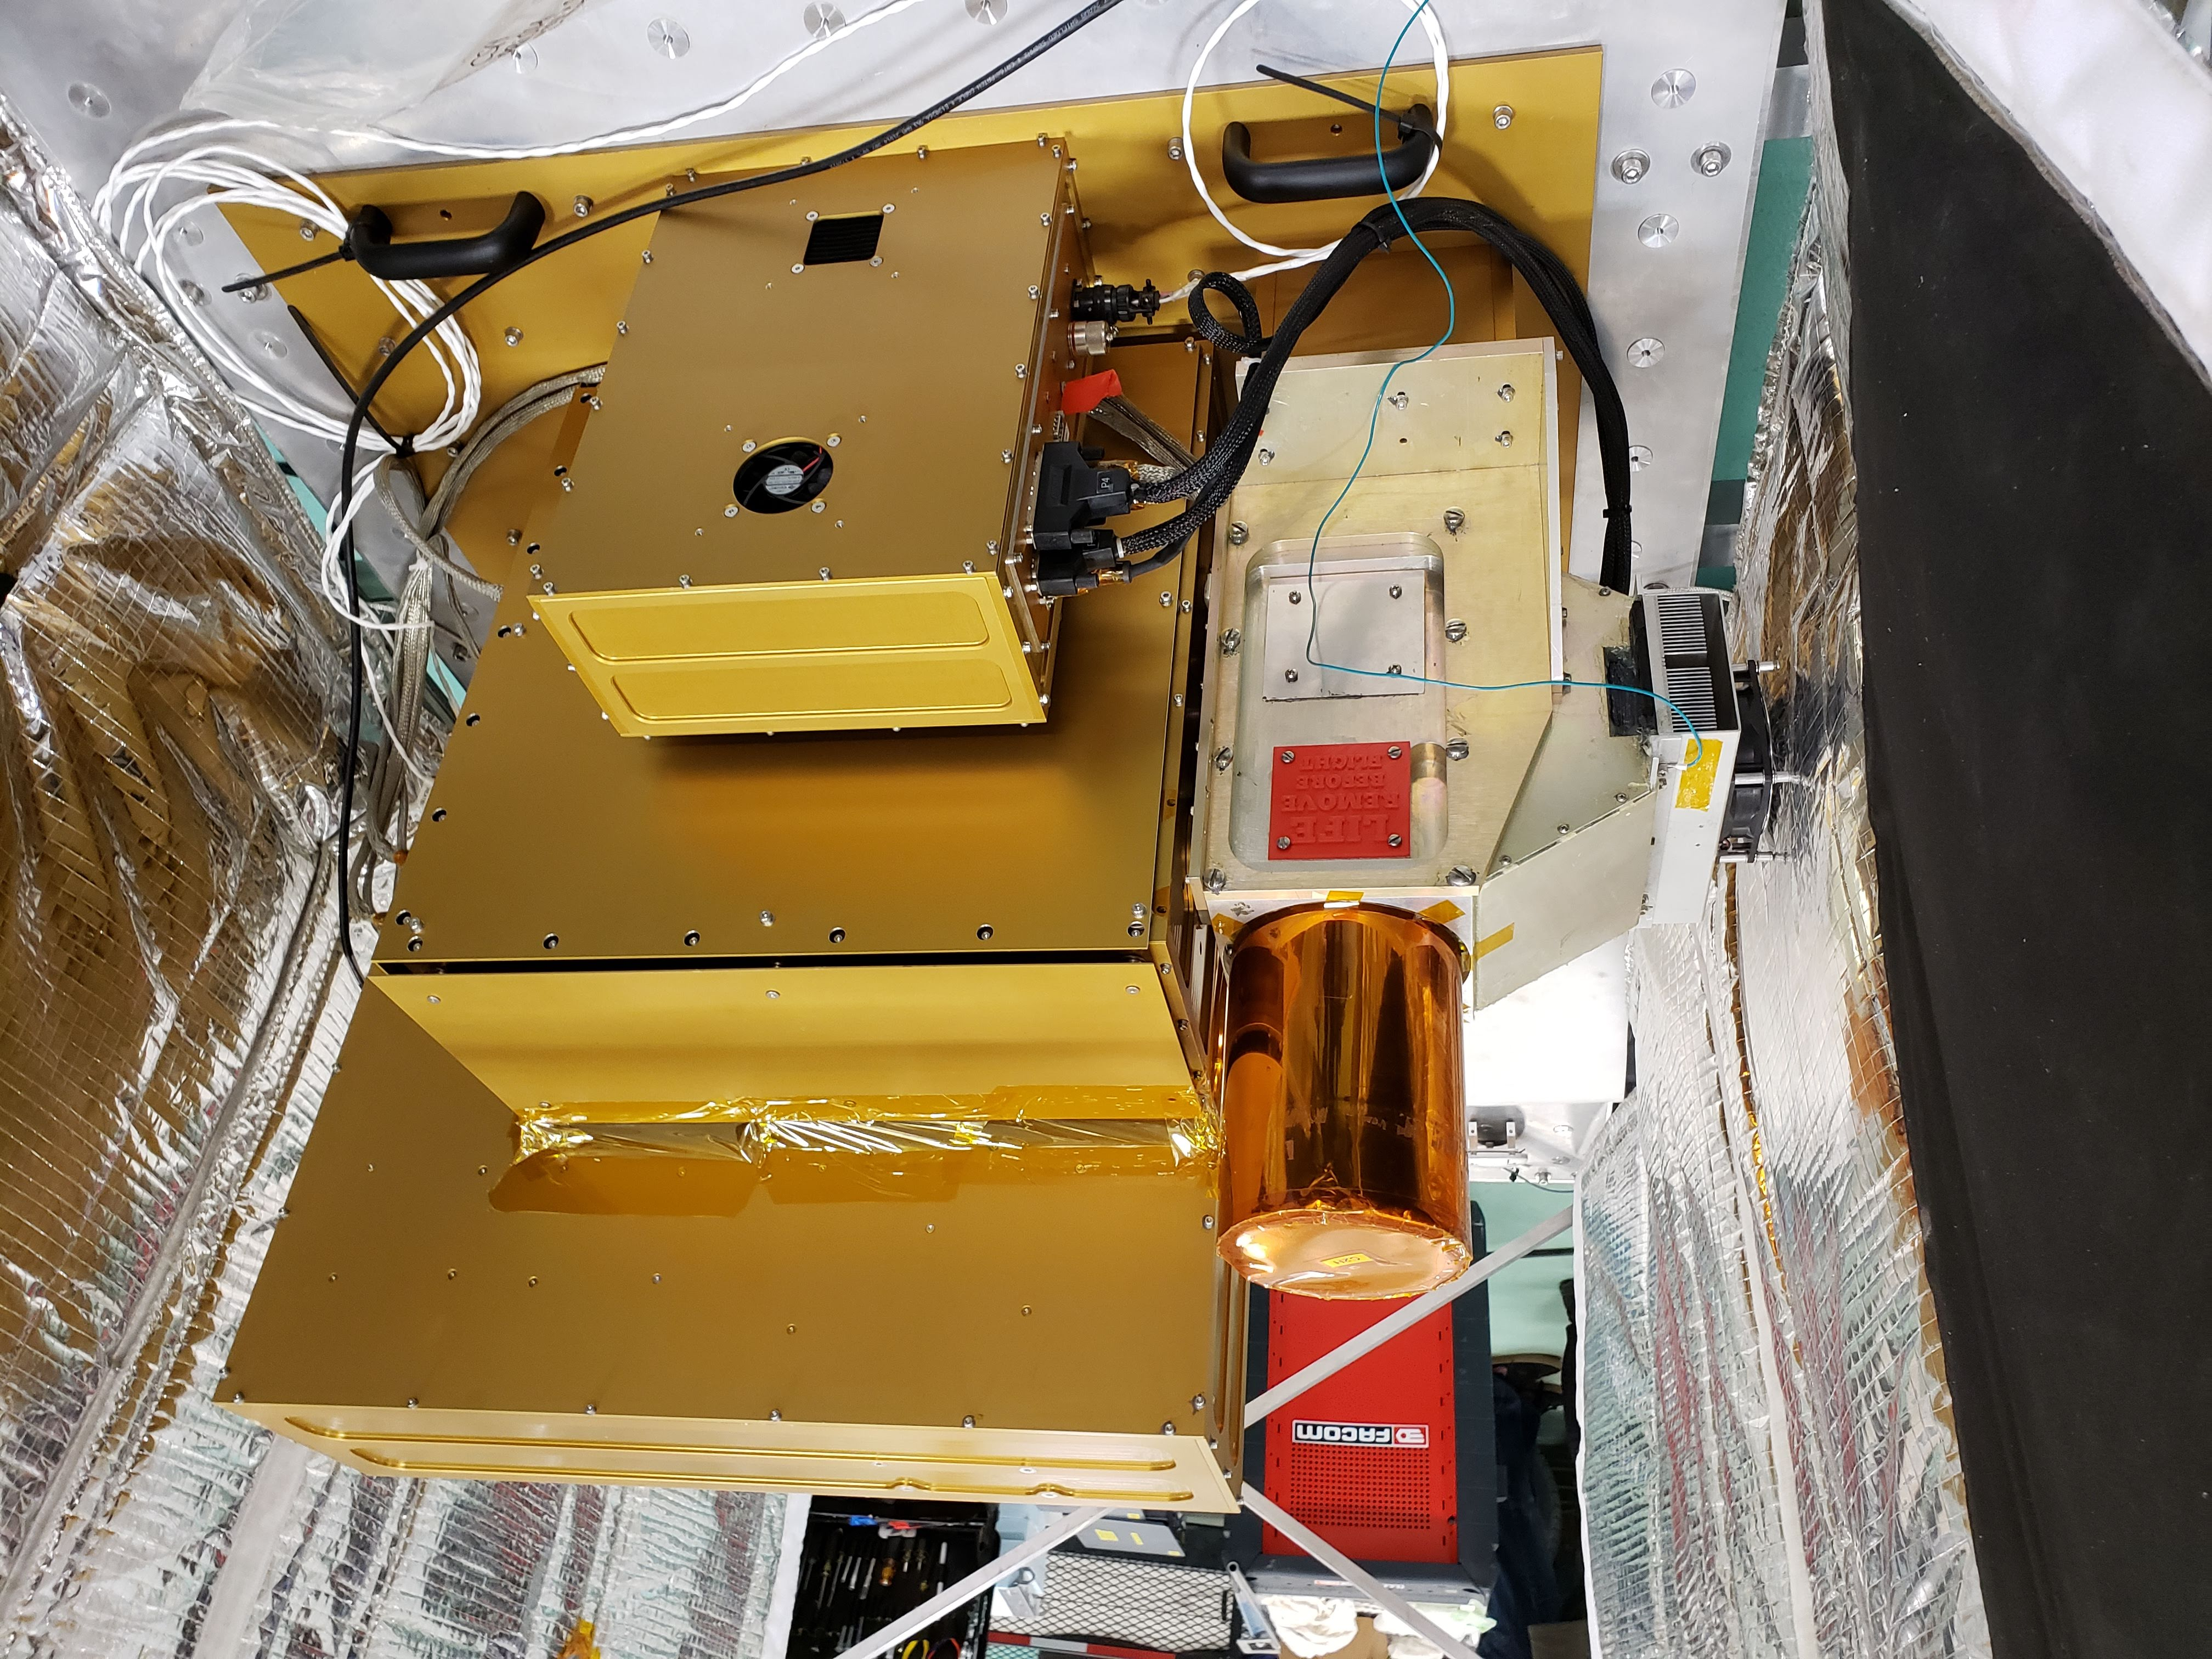
\includegraphics[width=0.7\linewidth]{chap4_images/LIFE_on_gondola.jpg}}
    \caption{LIFE integrated into the CNES gondola.}
    \label{fig:LIFE_ON_GONDOLA}
\end{figure}

The integration and checks all went smoothly. The instrument operated properly both through initial tests and while connected to the gondola. With this completed, the instrument was ready to launch, and would wait until the weather was clear and the CSA was ready to launch. This happened a week and a half through the campaign. The instrument was loaded onto the gondola at 7pm, initial checks and boot up was completed, final closures and connections to the instrument were made, and the instrument launched at 10pm. An image of the instrument sitting on the gondola waiting for launch and the inflation of the gondola balloon is shown in Figure \ref{fig:LIFE_BEFORE_LAUNCH}.

\begin{figure}
    \begin{subfigure}[h]{0.49\textwidth}
        \centering
        \rotatebox[origin=c]{270}{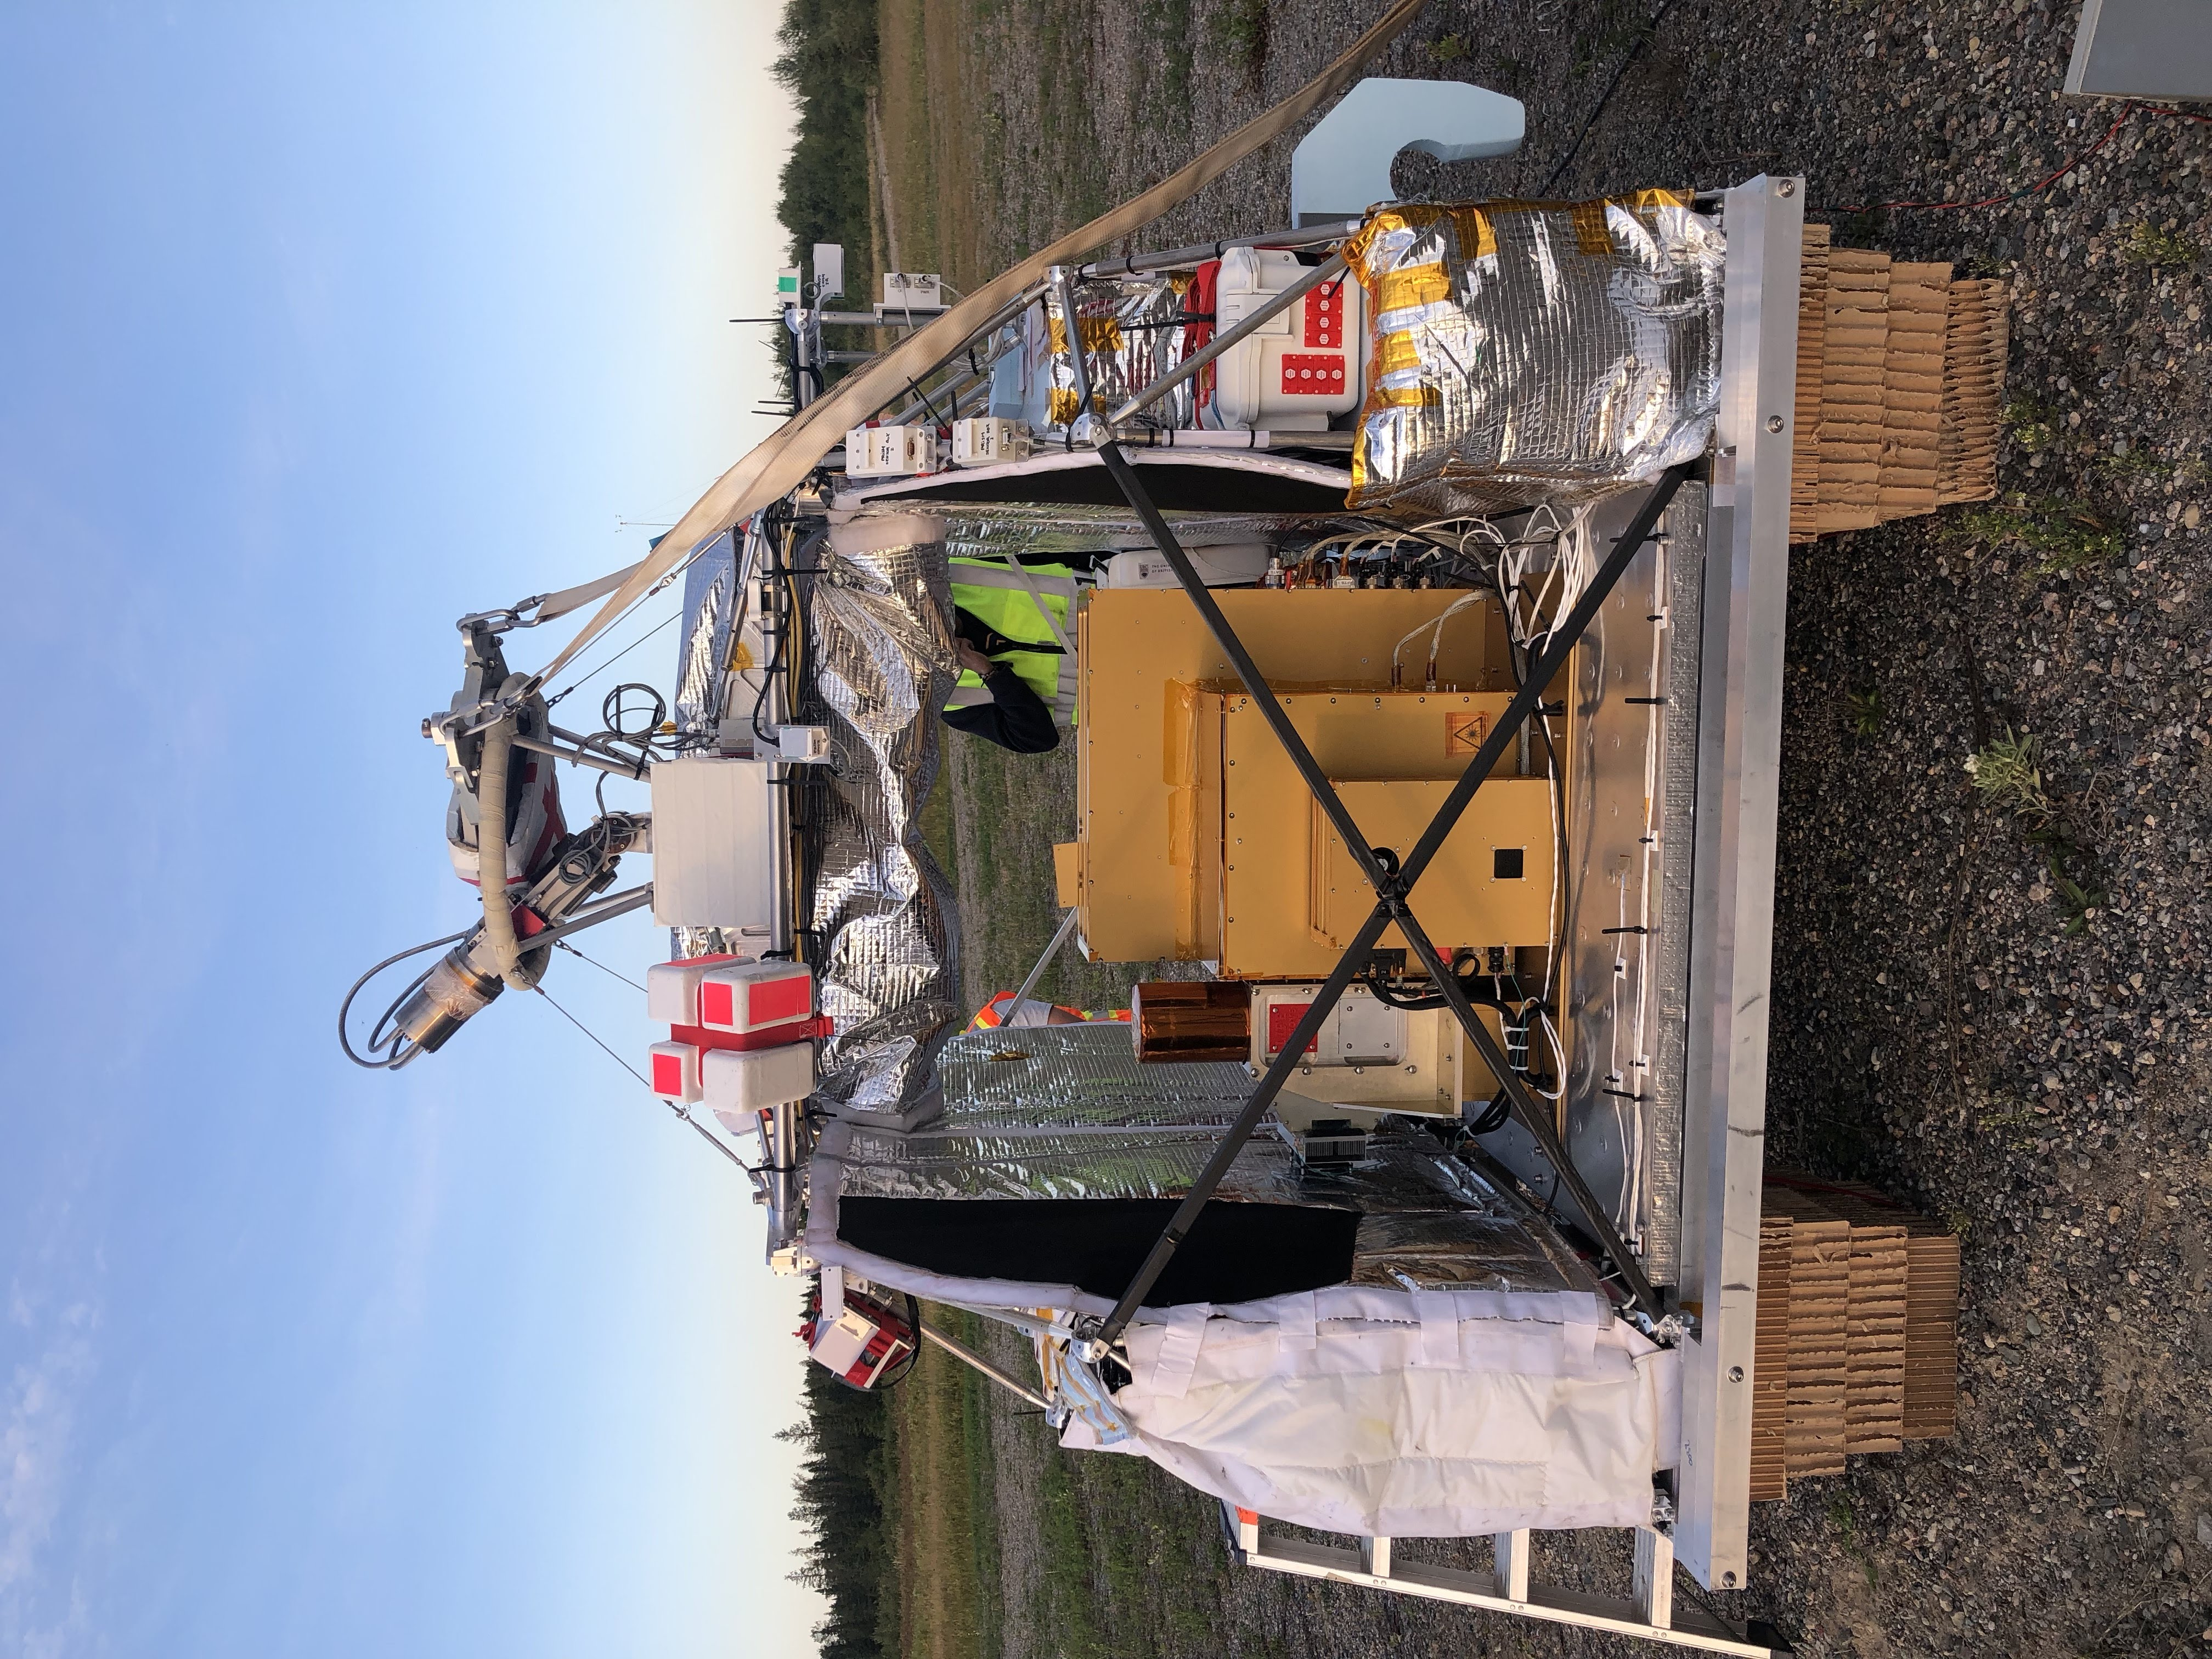
\includegraphics[width=\linewidth]{chap4_images/LIFE_on_gondola_2.jpg}}
        \caption{LIFE on gondola, on launchpad prior to launch.}
        \label{fig:LIFE_on_launchpad}
    \end{subfigure}
    \begin{subfigure}[h]{0.49\textwidth}
        \centering
        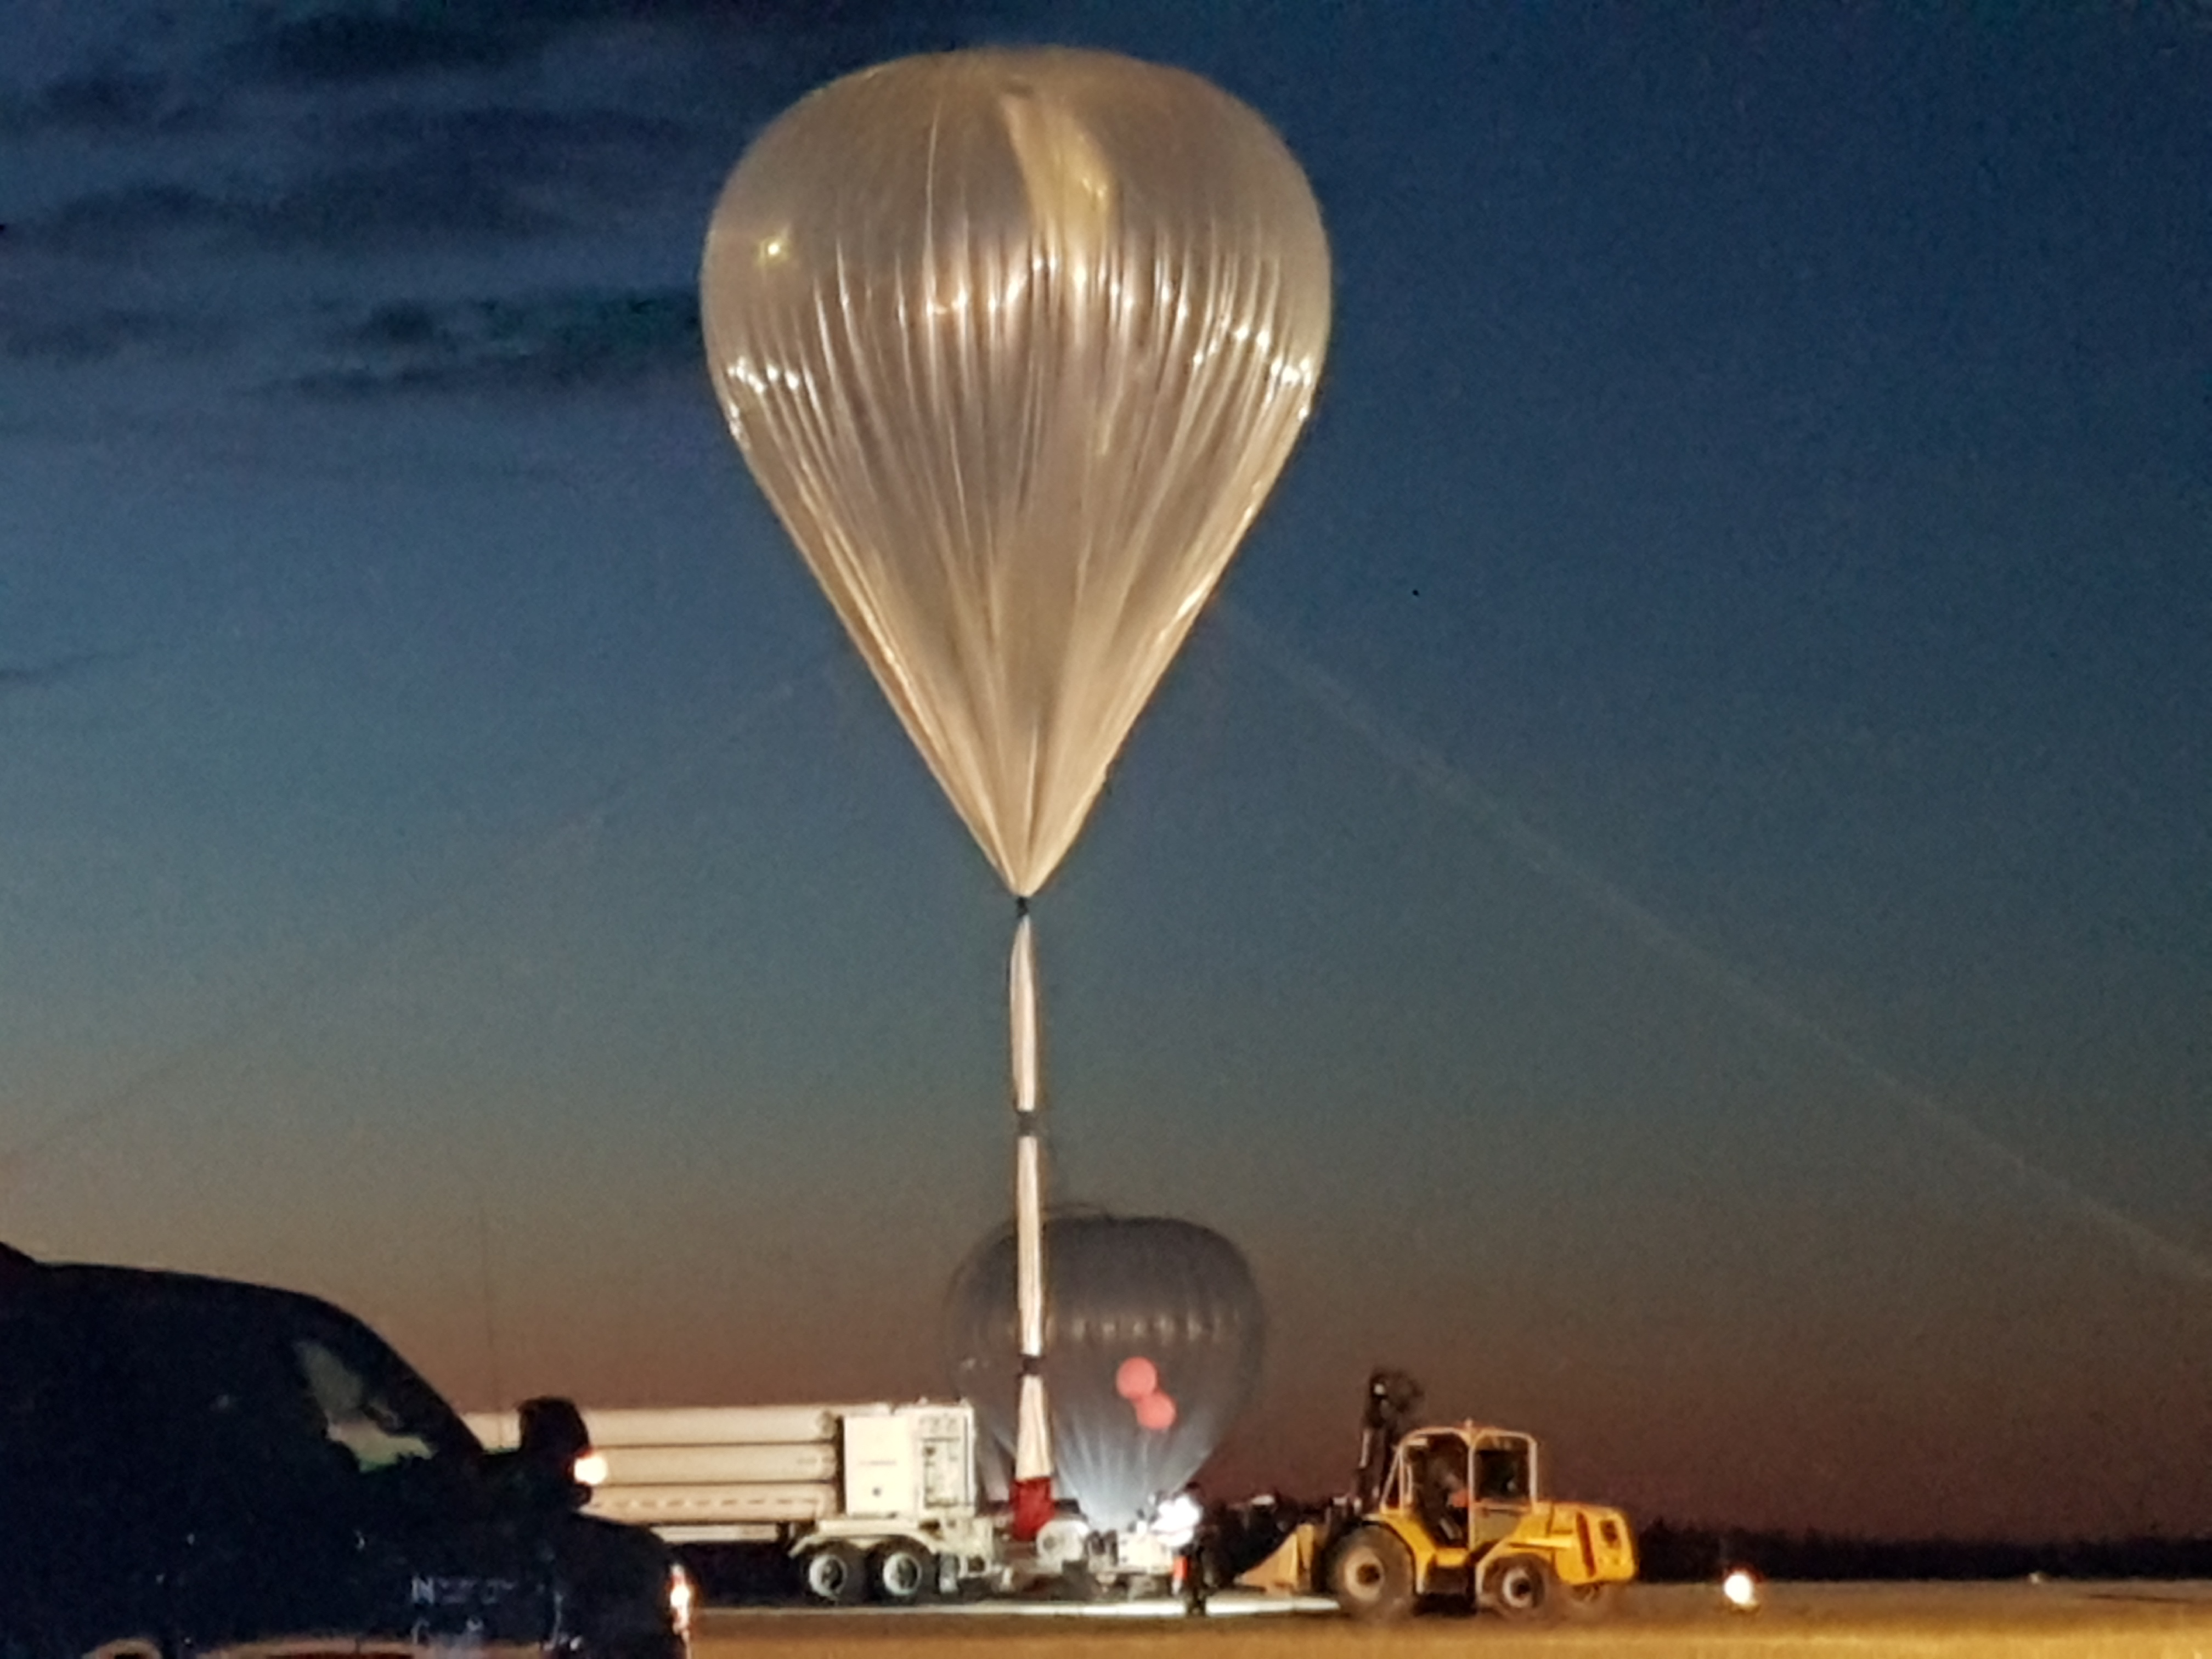
\includegraphics[width=\textwidth]{chap4_images/gondola_balloon.jpg}
        \caption{The gondola balloon being inflated shortly before launch.}
        \label{fig:gondola_balloon}
    \end{subfigure}
    \caption{LIFE being prepared for launch.}
    \label{fig:LIFE_BEFORE_LAUNCH}
\end{figure}

The instrument reached float altitude at roughly 1am. Measurements were taken throughout the ascent, but proper measurements could now be taken for the duration of the float. The instrument operated without issue through the entire float period. At about 5:30am, the sun rose, and the instrument began to warm. Initially, the CSA had no plans to operate the instrument in daylight, the gondola would be brought down prior to sunrise or shortly after. As this was expected, LIFE was shutdown at around 6am. However, CNES was having trouble finding a proper landing location that was not close to any water, which lengthened the flight. As the mission was extended, the team decided to reboot LIFE, so that more measurements could be taken, and thermal data could be taken while the sun rose. The sun has no effect on the data of the instrument, as long as it is not directly looking at the sun, the instrument can be operated at any time. Night was only chosen so that the thermal design could be simplified. The decision was made to operate the instrument until temperatures reached the maximum allowable temperatures. Normally, if the sunlight was expected, this would not be as much of an issue. CNES, if the gondola will fly during the day, installs sun-shields to shade the instruments to minimize the effect of the sun, but as this was planned as only a night flight these were not added. Thus the sun shining directly on the instrument contributed significantly to the heating of the instrument. The flight continued well into the morning, only coming down shortly after noon. Thermal data and measurements were successfully taken for an extra 6 hours past sunrise. This provided more data to try and model what the instrument would see when the sun rose, and is described later in this chapter. The instrument landed safely but fast in the early afternoon. An image of the instrument at its landing sight is shown in Figure \ref{fig:gondola_after_landing}. The results of this landing and the cause of its firm fall is described in the next section.

\begin{figure}
    \centering
    \rotatebox[origin=c]{270}{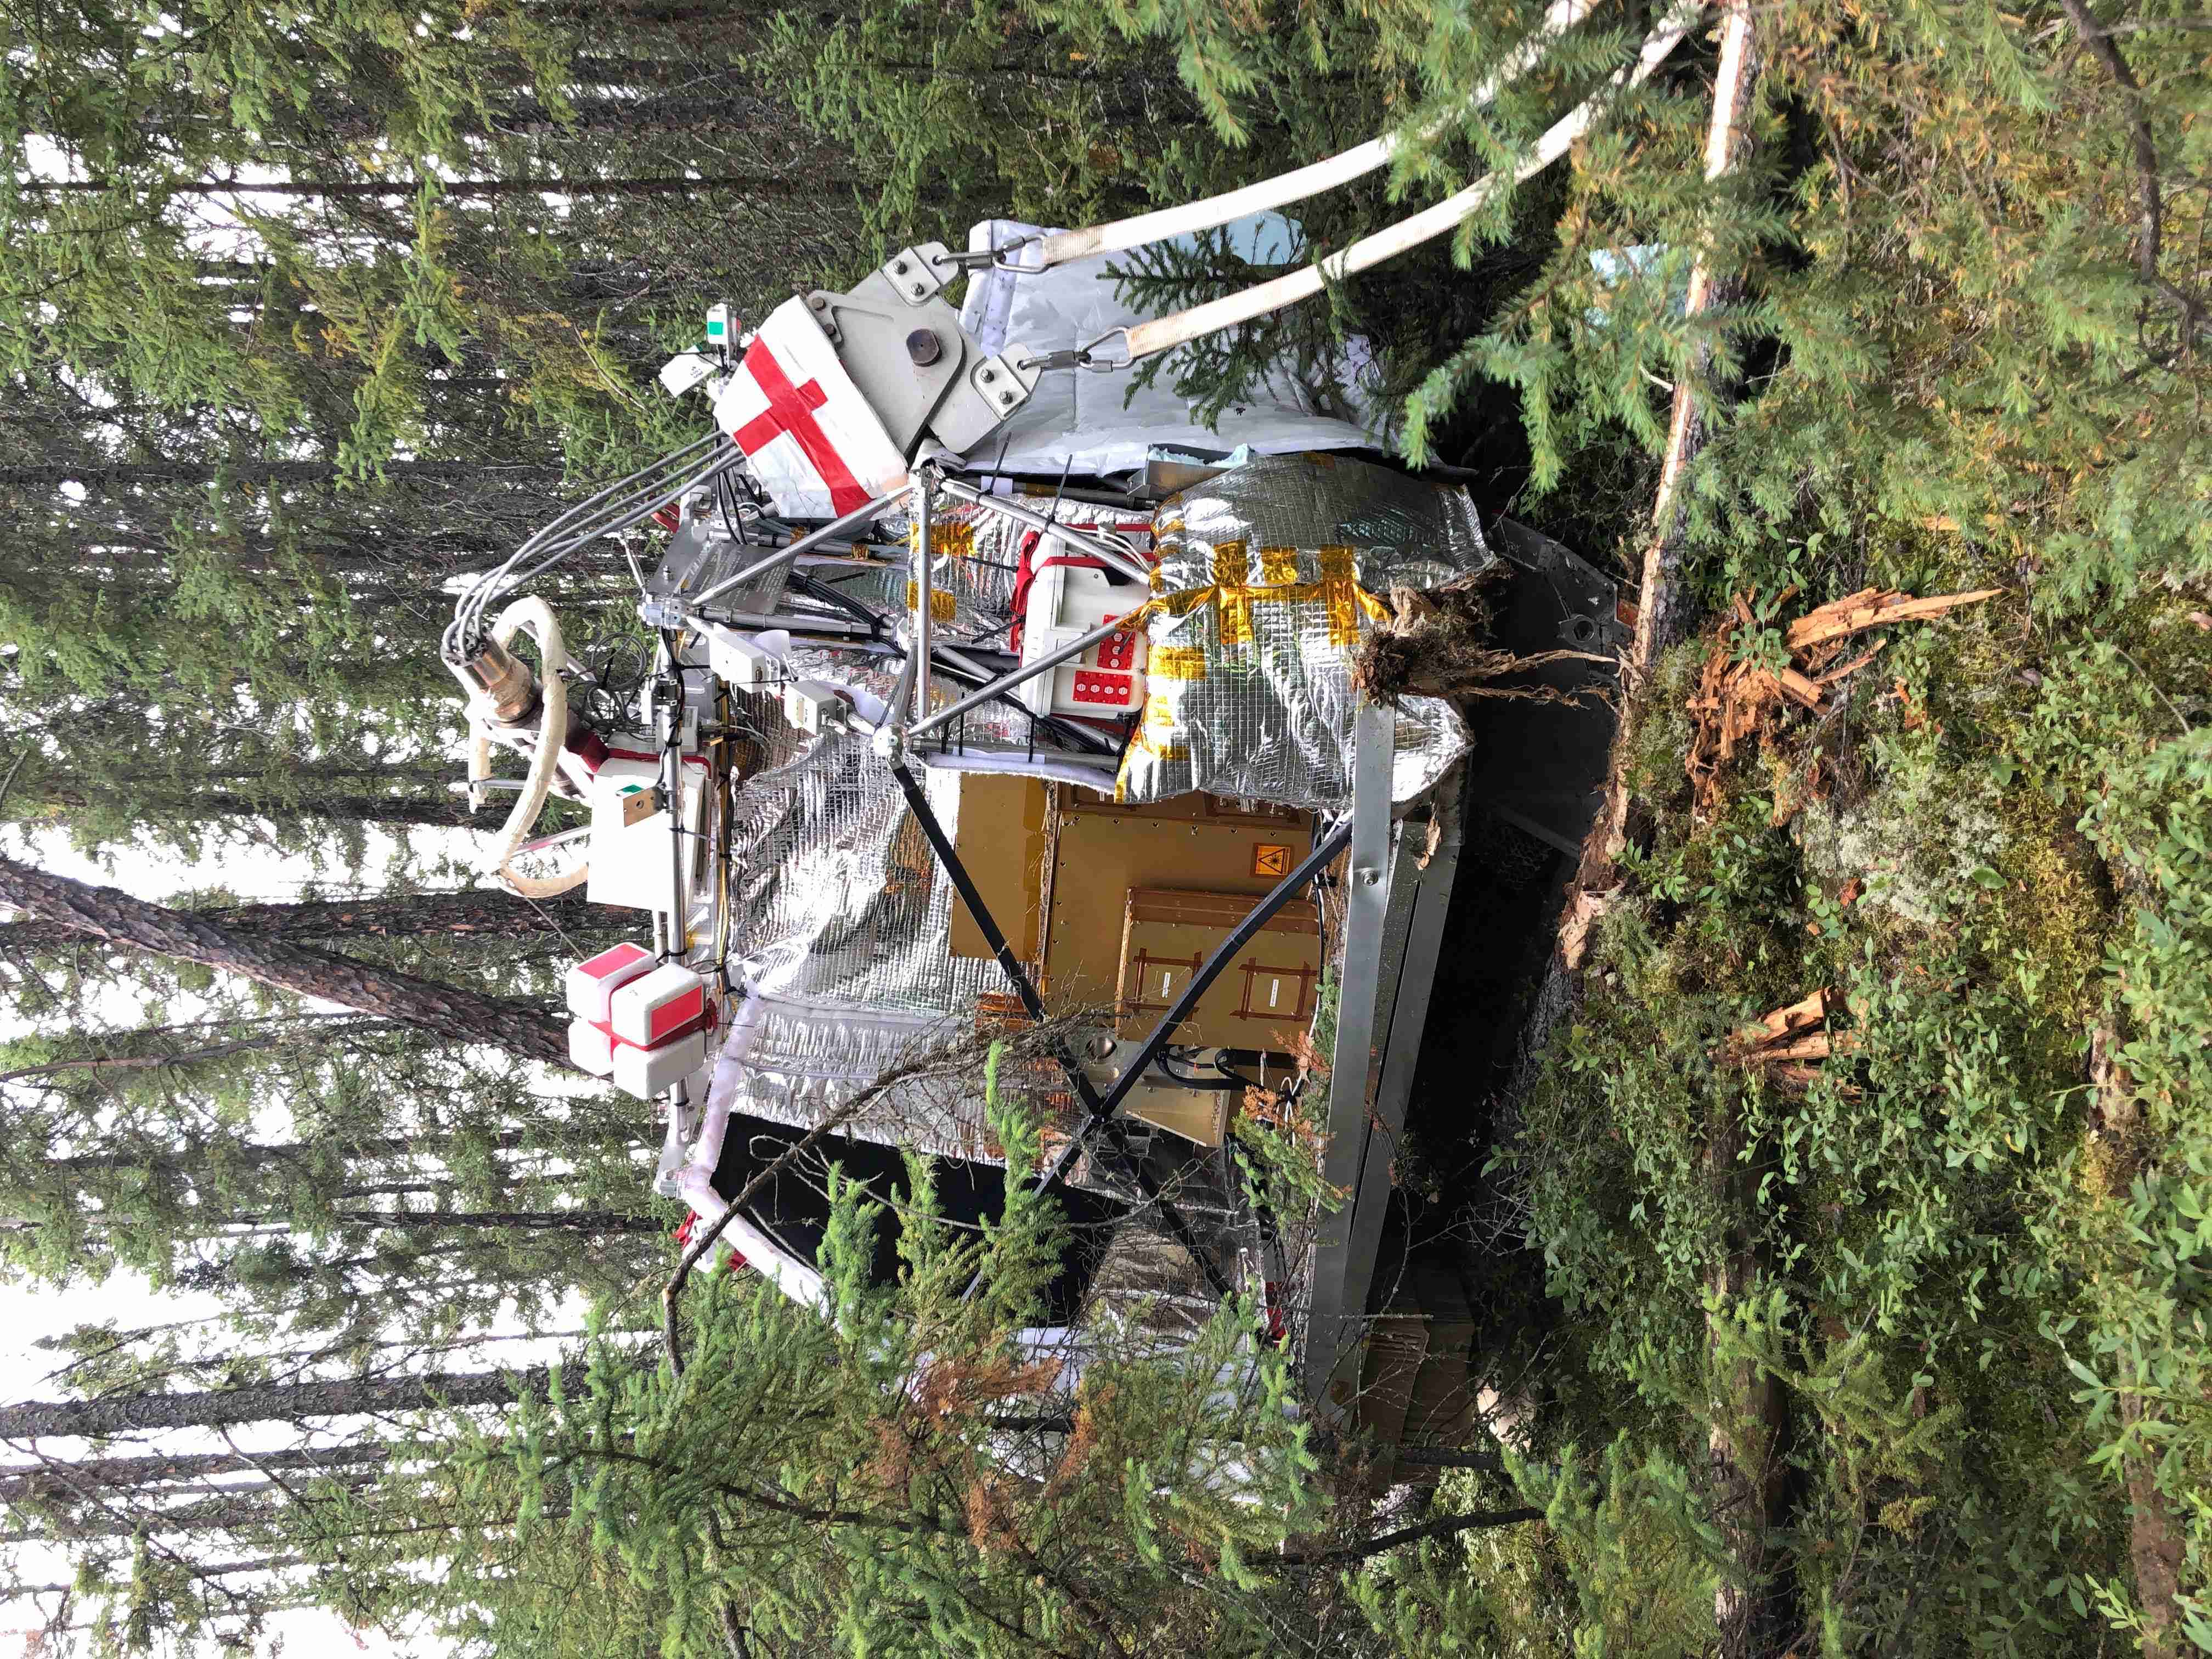
\includegraphics[width=0.5\linewidth]{chap4_images/gondola_after_landing.jpeg}}
    \caption{Gondola after landing.}
    \label{fig:gondola_after_landing}
\end{figure}

The instrument was recovered and was brought back to base by the next morning, and the team left the base shortly afterwards. When examining the data later, it was found that the flight had been successful. All images and measurements for the instrument were taken successfully, and thermal data of the instrument was successfully saved so that an accurate thermal model of the instrument based on this data could be created.

\section{Mechanical Results}
Although the flight overall was successful, the landing did not go as planned. For all gondola flights, the landing is the where the gondola is shocked the most, with a force of typically around 10-15g. This force is designed for and tested in the CSA mechanical verification spreadsheet, as discussed in Section \ref{Mech_changes}. However, on this flight, during the descent one of the parachutes did not open. Out of the typical three parachutes used during descent, only two opened properly. This caused two problems: One was that the gondola was descending much faster than was planned for. The second was that in addition to the descent speed, the gondola was falling at an angle, due to the three parachutes normally forming a triangle. Without the third, the weight was offset, and the edge of the gondola (towards the LIFE side) was going to hit the ground first, rather than the bottom of the gondola which was cushioned for the landing. The gondola eventually hit the ground with a shock that saturated the on-board force sensors at 20g.

This unplanned force did not cause any large structural damage. Even though the mechanical interfaces were tested to 15g, the safety factor helped the instrument survive over 20g. However, there was some evidence of the impact. The largest was that the bolts holding the Electronics Box to the instrument baseplate were stretched out, meaning that the Electronics Box was very close to breaking off. This would have caused the LIFE instrument to be totally destroyed, as the crucial connections between the electronics in this box and the detector in the Optics Box would have been destroyed as well. Thankfully this did not happen. An image of the result of the impact on this interface is shown in Figure \ref{fig:landing_damage_image}.

\begin{figure}
    \centering
    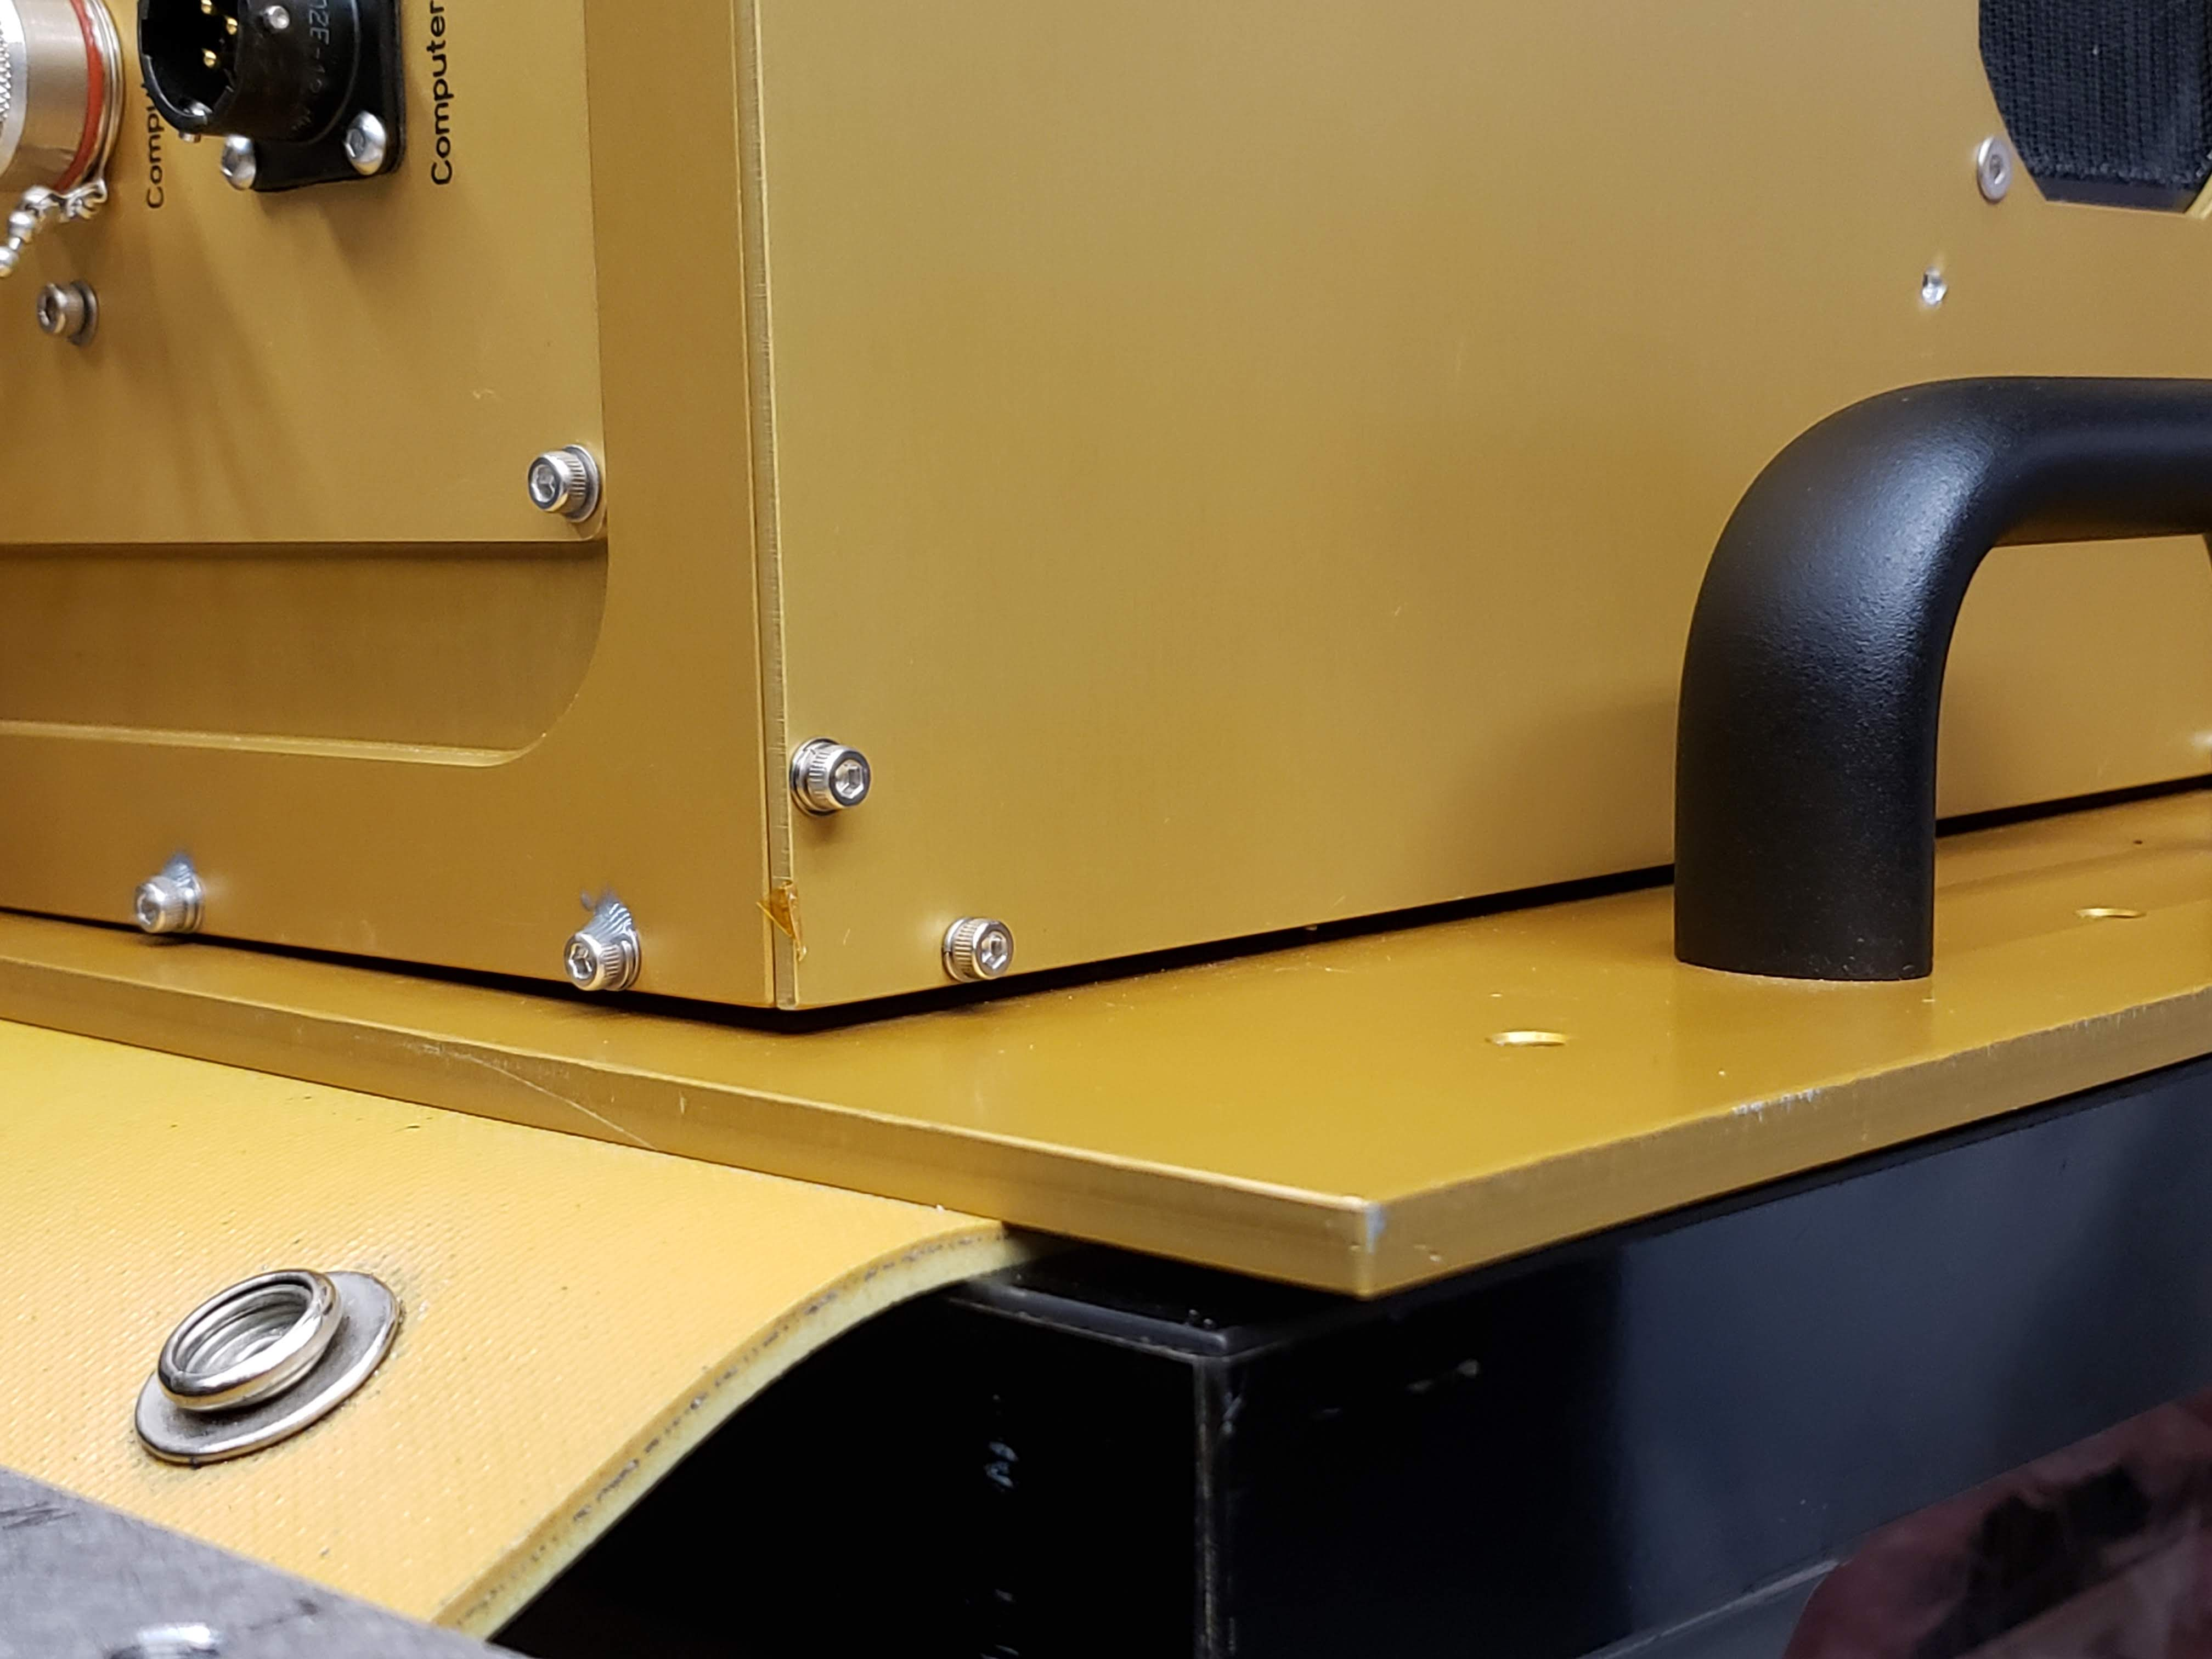
\includegraphics[width=0.8\textwidth]{chap4_images/LIFE_impact_result.jpg}
    \caption{A gap between the Electronics Box and baseplate, due to bolt stretching caused by the shock of landing.}
    \label{fig:landing_damage_image}
\end{figure}

This is one of the first things that need to be fixed prior to LIFE being used again. However, this was not the only damage caused. When the instrument was taken back to the university lab from Timmins to perform its post-flight tests, it was found that the detector could not reach the necessary measurement temperature of -198°C, not being able to move past -185°C. In addition, although images taken at -185°C are noisy but often usable, the images taken during these tests were much to noisy to be useful. There was an issue with the detector caused most likely by the landing impact. Through some data analysis on the noise during flight (described in detail in Section \ref{detector_noise_flight}), and eventually removing the detector to send it to the manufacturer, it was discovered that the cold stop of the detector was now no longer attached to the Stirling cooler. Thus it was not being cooled properly and could not be used. There is a very high cost in repairing the detector so that the instrument may be able to be used or modified for further missions, and it is unsure whether is will be fixed. As a result, no post-flight tests could be done to perform further verification and testing of the instrument.

\section{Flight Temperature Model}\label{flight_temp_model}
After the flight was completed, the temperatures seen during flight were compared to what was seen in the model. The most important aspect from the thermal-mechanical design was that everything stayed within its required temperature ranges for the float part of the flight, when everything was operating as needed. However, the temperatures did not match what was seen in the tank, for a variety of reasons, but mainly because there are so many variables in high-altitude balloon flights. It is difficult to make an accurate model, even for just the simplest parts of the flight, because there are a number of variables that may effect the temperature, and next to none are documented or studied. For example, there is no information on how convection changes as altitude increases, especially at altitudes above the troposphere, and not for the temperatures seen. There is no information on the precise amount of solar heating on an instrument that is dependent on altitude. A number of other questions also remain.

As a result, it was decided that as part of this thesis, a temperature model of LIFE would be created, for all stages of flight. Through numerous simulations and different values for different thermal phenomenon, the temperatures of different parts of the instrument in the simulation would be made to match the temperatures seen during flight. This would include all phases, not just the float, which is the easiest and was modeled prior to flight. This model could then be a basis for all future high-altitude balloon instruments to draw from, for thermal simulations and what to expect during a flight. This will helps to ensure better survivability in future instruments.

Of course, there are too many variables to use this thermal model for all future instruments as is. It is meant to provide a starting point, and can help to plan for what to expect beyond ensuring that it will survive when the base of the instrument is cold. It can help to plan for the fast temperature decreases seen through the ascent, and help to design for better protection of the instrument should it be running in daylight. And through future missions, the model can be improved through new thermal data, until a thermal model with multiple flights of temperatures and improvements has been made can be used on future instruments with little changes. This will help to reduce the workload on future instruments and reduce costs and engineering time. 

Before going further into the temperature simulations, the flight temperatures as a whole is examined in more detail. A plot of the flight temperatures measured by both the LIFE temperature sensors and a temperature sensor on-board the gondola baseplate is shown in Figure \ref{fig:full_temps_no_sims}. The altitude of the gondola is also shown in this figure.

\begin{figure}
    \centering
    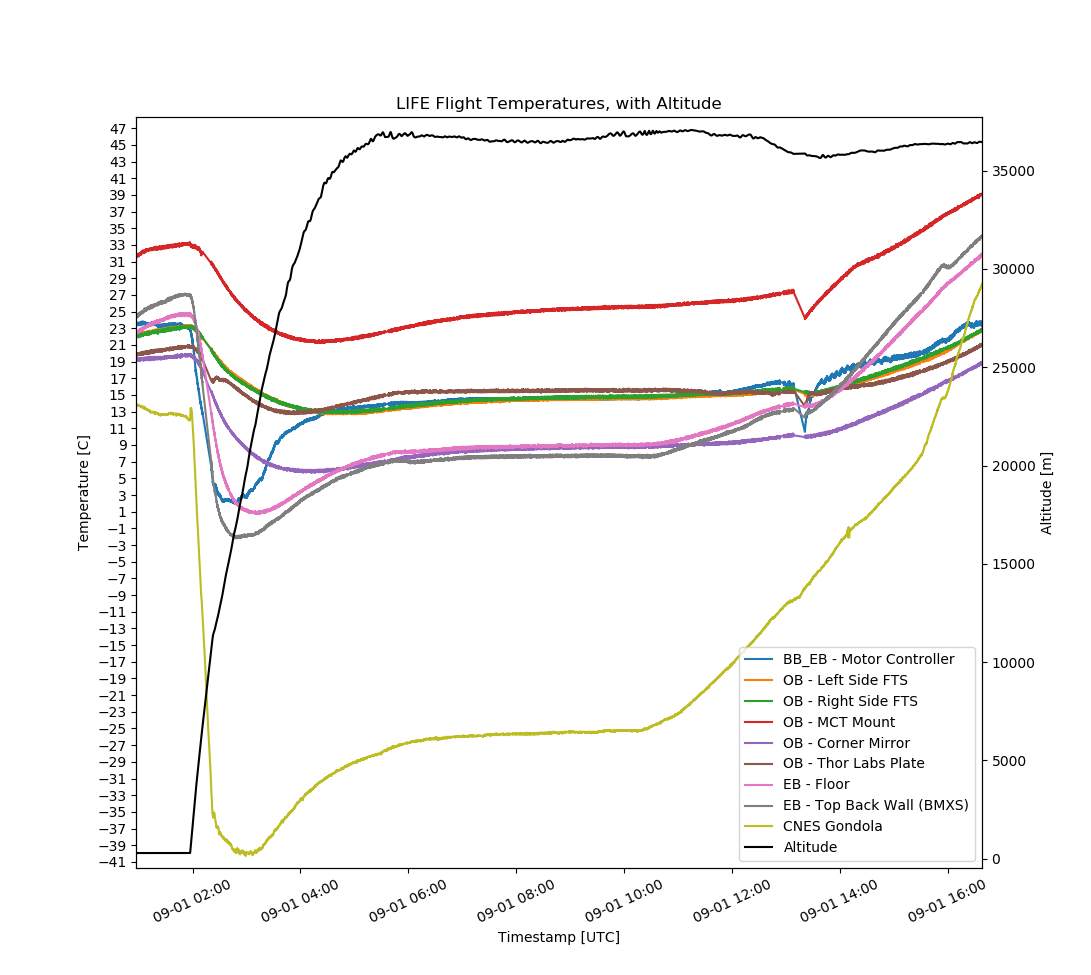
\includegraphics[width=\textwidth]{chap4_images/full_flight_no_sim_temps.png}
    \caption{Temperatures over the course of the August/September 2019 Timmins flight.}
    \label{fig:full_temps_no_sims}
\end{figure}

Described here at a high level, with more detail in subsequent sections, the different phases of the flight can be seen here. The initial linear increases in temperature is from the instrument heating up as it sits running and waiting for launch on the launchpad. The increase in temperature is due to the lack of fans, which needed to be turned off and covered prior to flight. Immediately following launch at 2:00 UTC, the temperatures drop dramatically. This is the result of the cold region of the tropopause quickly cooling the instrument; on the night of the LIFE launch, the tropopause region was at roughly -50°C, which the gondola travelled through for almost half an hour. The instrument begins to warm once it reaches the warmer stratosphere. The gondola stabilizes just above 35km at roughly 5:00 UTC, where measurements are taken.

Through the main measurement phase of the flight, from 5:00 to 10:30 UTC, the temperatures are extremely stable. The maintain the required temperature drift through this time frame, only changing once the instrument begins to heat from the sunrise. All temperatures are also in their required ranges, with the optics staying just below 15°C and the electronics staying in the 5-10°C range. This is slightly cooler than expected, which is due to the initially cold temperatures from the ascent. At the end of this phase, the sun begins to rise, and temperatures begin to rise as well. A small dip shows where the instrument was momentarily turned off, and the flight was expected to end. When it was turned back on, the instrument had cooled slightly, but began to rapidly warm due to the electronics and sunlight, until everything was finally turned off at 14:30 UTC. 

The goal for the thermal model is to match the simulated temperatures to what is seen in Figure \ref{fig:full_temps_no_sims} through a series of iterations. For the purposes of the simulation, the flight was split into three major phases: The ascent through the troposphere and tropopause, the float period when the instrument is at altitude and taking measurements, and the sunrise, when the sun begins to shine on the instrument and have a major effect on the temperatures. Each of these simulations were completed one by one, and the final temperatures of each simulation made to match precisely what was seen during flight. These final temperatures of a simulation would be used as the initial temperatures of the next simulation, so was important that they were very close to the actual temperatures to avoid temperature propogation errors. Once the final temperatures were met, the temperature curve of each section was compared to the temperature curve of the flight and different inputs of the model were iterated through.

\subsection{Ascent}\label{ascent}
The first part of the flight was the ascent. This included the rise from ground level, up through the tropopause, and into the float level of 35km in the stratosphere. This was the most difficult part of the flight to simulate, because this part has the most variables and the most change in temperatures. Convection only plays a role in this part of the flight, and is the biggest unknown that will need to be determined. Radiation with the rapidly changing temperatures, conduction with the rapidly changing baseplate temperature, and forced convection as a result of the speed of the rising balloon gondola all need to be considered for this part of the simulation. As a result, it is likely the least accurate part of the entire thermal model, and also required the most iterations to model correctly.

\subsubsection{Measured Temperatures}
The simulation was split into two halves: The ascent up until the troposphere, and the ascent past the troposphere up to the stratosphere. The centre of this split is the temperature minimum for all components. The time of the launch was 2:00 UTC. The time until the temperature minimum, or when the gondola left the tropopause and began to warm up again, was roughly 3:00 UTC. The second part of the ascent, which ended when the gondola stabilized at the float altitude of 35km, was from 3:00 to 5:00 UTC. The temperature measurements of the entire ascent phase of the flight along with the altitude during this time is shown in Figure \ref{fig:ascent_temps_no_sims}.

\begin{figure}
    \centering
    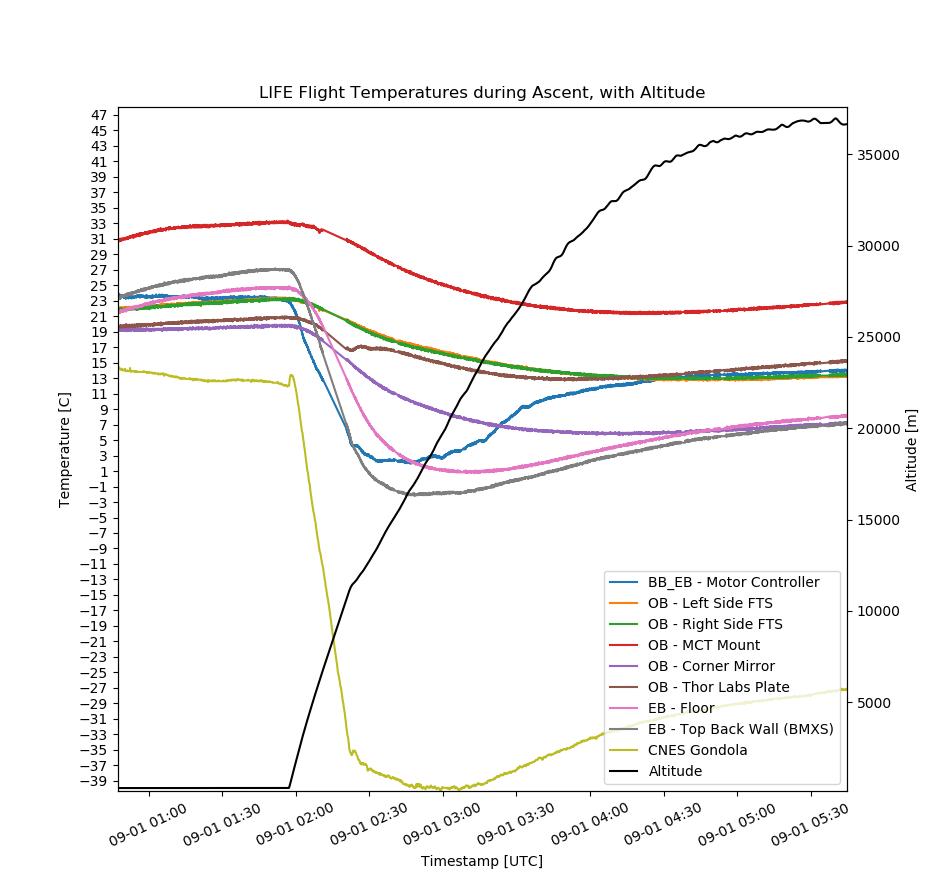
\includegraphics[width=\textwidth]{chap4_images/ascent_images/ascent_no_sim_temps.png}
    \caption{Flight temperatures through the ascent, the first three hours of the flight.}
    \label{fig:ascent_temps_no_sims}
\end{figure}

For the hour leading up until launch, the instrument is sitting on the launchpad, powered on and waiting; this is where the temperatures are slowly increasing. The most important part of this phase is the temperature drop shortly after launch. The cold air has the largest affect on the gondola baseplate, which drops to -40°C by the end of the tropopause, and overall it drops 50°C in as little as half an hour. This is the result of the cold air and the forced conduction at these speeds and altitudes. As the LIFE temperature sensors are inside the boxes, the temperature changes are slightly delayed. The effects of the isolation of the Optics Box is evident here. The three sensors that show the largest and quickest temperature drop are either in the Electronics Box or the Blackbody Electronics Box, which are not insulated from the baseplate. The lowest temperature seen anywhere on-board LIFE is just below 0°C, where the top of the Electronics Box dips due to the effect of convection on the largest open plate in the instrument. Unfortunately, this was one of the few parts of the instrument that dropped outside of its required temperature range, but quickly warmed again from the heaters powering on, and no cold damage was sustained. Once the environmental temperature warmed and the heaters fully powered on, the temperatures quickly increased back to nominal.

All optics components show a much slower temperature decrease, as they are slowly cooled through the two layers of thermal insulation of the titanium spacers. Instead of dropping quickly and warming from the heaters, these components slowly decrease until they begin to stabilize from the warmer temperatures outside the box and the optics plate heater maintains the required temperatures inside the box. These temperatures, as long as heater power to this heater as well as the other electronics heaters, were monitored closely through this phase of the flight to ensure temperatures were not dropping to quickly and the temperatures were being maintained towards the end of the ascent.

\subsubsection{Simulations}
With the ascent temperatures fully described and understood, a thermal model was then developed to attempt to match these temperatures. All thermal loads are described here, and the decisions and iterations behind each. Through 30 iterations for the first half of the ascent and another 31 for the second half, each thermal load was examined and tweaked. There are a total of 41 thermal loads in these simulations.

An important and difficult aspect of this first stage was the initial temperatures. Because the instrument had been running on the launchpad for an hour prior to launch, different components were at different temperatures as a result of the electronics. For example, the MCT detector dumps a large amount of heat as it cools, and this was sitting at above 30°C as the instrument was launched. In a SolidWorks thermal simulation, it is very difficult to choose initial temperatures for different components. Most often, the entire instrument has one initial temperature, and if not then each component of the entire assembly must have its own initial temperature. In the thermal model, this is upwards of 1000 components. One of the motivations for creating the ascent temperature model was to provide accurate initial temperatures for the float component of the flight without having to choose each of these separate initial temperatures. To avoid having to simulate the instrument sitting on the launchpad to get these initial temperatures, an average of the core component temperatures was taken, which was 23°C. This temperature was then applied to all components. 

The next thermal property discussed is conduction, which is also the easiest as the environment has no effect, unlike radiation or convection. Discussed previously in Section \ref{final_pre_flight_sims}, the biggest unknown with conduction is the thermal conductivity across mechanical interfaces. A large aspect of the TVAC simulations and thermal comparisons were determining the actual values for these conductivites. Through these tests the conductivity for the boxes to the baseplate (two anodized surfaces) was found to be 0.16 $w/m^2K$, and the conductivity for the optics components to their mounts, and their mounts to the baseplate (anodized to bare aluminum surfaces), was 0.20 $W/m^2K$. These conductivites were not changed for the flight, and are used in all flight simulations.

Radiation of various surfaces of LIFE is a large problem in the simulations. To be able to simulate radiation, three values are needed: The view factor to other surfaces, the emissivity of the surface, and the temperature of nearby surfaces. The emissivity is the most well known property of these three values, and does not need to be tweaked. The three most common materials and surfaces all have well known emissivities: Anodized aluminum, which is the majority of the box components as well as the optics breadboard, has an emissivity of 0.77. For circuit boards, the emissivity of silicon is 0.6. Bare aluminum, such as the for parts of the blackbody system, has a very low emissivity of 0.05. 

The other two properties needed for radiation are much more difficult to determine. However, the view factor was slightly easier as it stayed constant through all simulations, so once good values were found in the initial ascent phase simulations then they did not need to be changed again. As described in Section \ref{radiation_sec}, the view factor can be calculated automatically through the simulations, but due to the complexity of the view factor integral equation, it dramatically increases the solve time, the the values are estimated and entered manually. Each radiative surface must be assigned a view factor to another surface at a certain temperature, and the view factor is a number representing the percentage of the surface that can be seen, from 0 to 0.99. Some of these estimations were simple, such as the outer surfaces of the boxes to the inner gondola walls. As there was nothing obstructing the view between these two surfaces, they would have a higher view factor, above 0.9. Similar estimations could be made between the electronics surfaces in the Electronics Box to the box wall.

However, many surfaces proved more difficult. For example, a difficult surface to estimate was the optics breadboard. As certain sections of the component have different view factors, the component that will have the largest effect is chosen as the comparison. With the breadboard, it would be the wall of the Optics Box. However, this would not take into account all of the optics that are mounted on the breadboard and are between these two surfaces, all of which are at different temperatures. Similar decisions needed to be made for interfaces between box walls, and the inner surfaces of boxes were electronics are mounted.

The most variable component of the radiative heat loads was the ambient temperature. For all previous tests, such as the TVAC and initial test simulations, these temperatures were constant, as the environmental constraint temperatures were held constant. However, with the rapidly changing environment for the ascent, the ambient temperatures rapidly change. Thus, a temperature curve must be created and input into Solidworks. This had to be done for all major components, and the curve was roughly modelled after what was seen during flight, and the known temperature of the atmosphere at increasing altitudes. This could be accomplished easiest for the outer surfaces of the instrument, especially those that viewed the atmosphere, as this temperature was well known. More complex were the outer surfaces of the instrument that viewed the insulated walls of the gondola, which were a reflective insulation material which would have different temperature effects. The ambient temperatures for interior components and surfaces needed to be chosen based on both measured flight temperatures and what the temperatures were from previous iterations of the simulations. One of the most difficult parts of choosing these temperatures was that if the ambient temperature was changed, to reflect a temperature change from the latest version of the iteration, it could have rippling effects causing more temperature changes in future iterations. In short, changing the ambient temperature of one part to reflect another could change the ambient temperature seen, and it would need to be updated again for the next iteration. This is one reason why so many iterations were necessary. An example ambient temperature curve is shown in Figure \ref{fig:ascent_pt1_top_box_rad}, for the first hour of the ascent for the external box surfaces. A curve like this is created for almost every radiating component in the model.

\begin{figure}
    \centering
    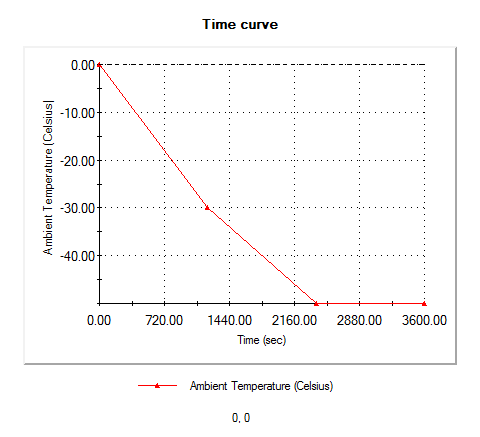
\includegraphics[width=0.7\textwidth]{chap4_images/ascent_images/ascent_pt1_top_box_rad.png}
    \caption{An example of creating the ambient temperature curve for the radiation of a component, specifically for the top surfaces of the boxes for the first half of the ascent.}
    \label{fig:ascent_pt1_top_box_rad}
\end{figure}

Finally, the last remaining and likely most difficult heat load is convection. This is the most complex and hardest part to model because it has two features, with unknown values, that both change with time. The first is the convection coefficient, or how quickly heat is flowing to or from the surface as a result of the convection. It is extremely difficult to calculate, and even if a value is calculated the error is much too large to be able to use confidently. In addition to the convection coefficient, the ambient temperature must also be varied throughout the simulation, in the same way as it is for radiation. This value was at least partially known, through the temperature sensors from flight and from the known temperatures of the atmosphere. The convection coefficient however would be roughly estimated and changed numerous times.

The convection coefficient of air can be anywhere from 1-10 $W/m^2K$ for free flowing air, and anywhere from 1-100 $W/m^2K$ for forced convection. It also drastically changes with pressure, as there is less density of fluid to be able to transfer heat. As discussed in Section \ref{convection_sec}, there are very few studies of the effect of pressure on convection, and only for the purposes of high heat industrial processes. As there was no information for a high altitude balloon scenario, information was taken from the forced convection scenario, and steadily decreasing as a result of the decreasing pressure. For the exterior parts of the instrument, forced convection would be the most prevalent. However, as the gondola was mostly covered, the forced convection would likely not be overly strong. An estimation of 10 $W/m^2K$ was made as an initial value, and steadily decreasing to zero by the end of the first half of the ascent. The pressure past the tropopause is estimated to be too low for convection to have any effect past this point. Convection was estimated inside the boxes to be between 1-5 $W/m^2K$, as the enclosures would limit any forced convection due to moving air from the ascent. Overall, these convection loads only played a part in the first part of the ascent, with the exception of some small convection on the bigger surfaces for the second part of the ascent. The ambient temperatures were kept the same or similar as the values used for radiation, to make the iterations simpler and for continuity across all components.

\begin{figure}
    \centering
    \begin{subfigure}[h]{0.9\textwidth}
        \centering
        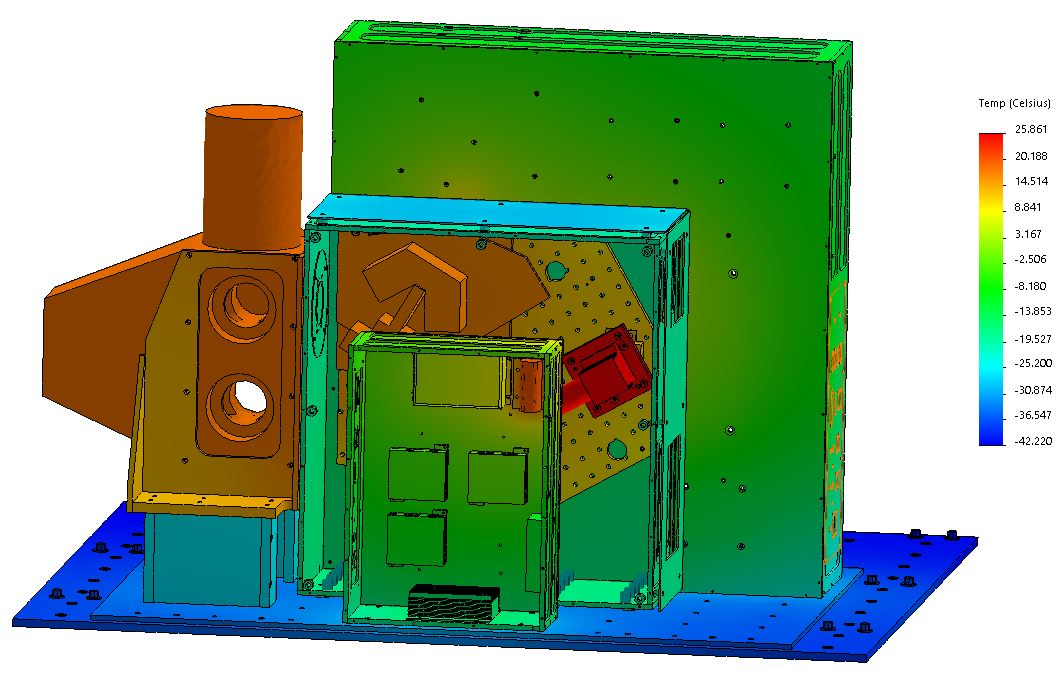
\includegraphics[width=\textwidth]{chap4_images/ascent_images/ascent_pt1/Test_30_BBEbox.JPG}
        \caption{Thermal model of LIFE instrument after the first hour of flight, Blackbody Electronics Box view.}
        \label{fig:ascent_pt1_model_bbebox}
    \end{subfigure}
    \begin{subfigure}[h]{0.9\textwidth}
        \centering
        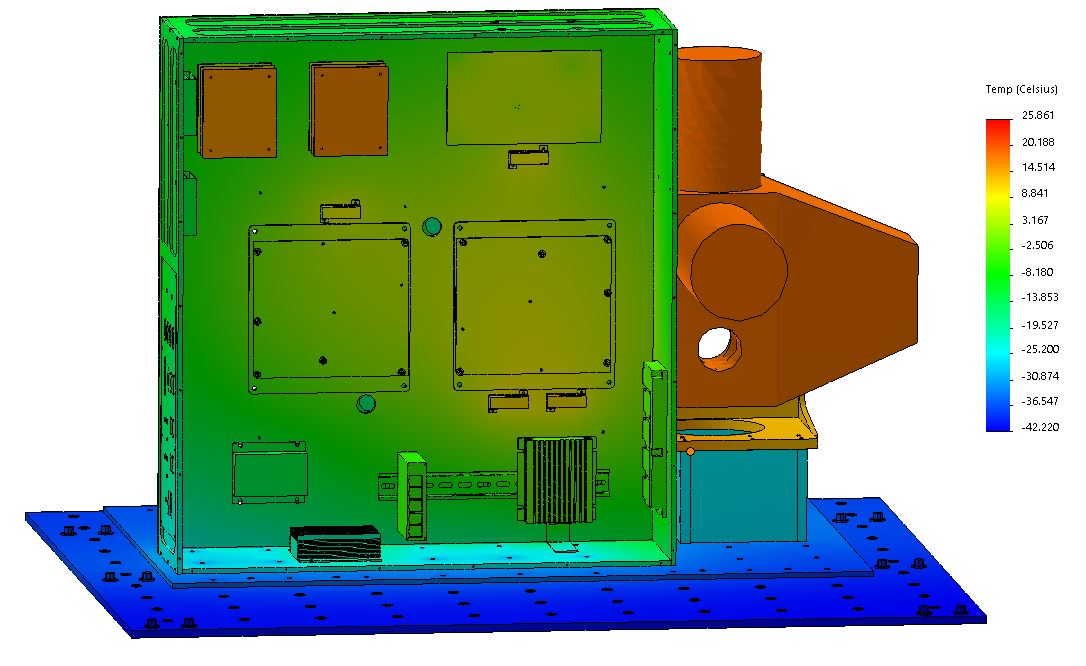
\includegraphics[width=\textwidth]{chap4_images/ascent_images/ascent_pt1/Test_30_Ebox.JPG}
        \caption{Thermal model of LIFE instrument after the first hour of flight, Electronics Box view.}
        \label{fig:ascent_pt1_model_ebox}
    \end{subfigure}
    \caption{LIFE thermal model following first half of the ascent.}
    \label{ascent_pt1_model}
\end{figure}

\begin{figure}
    \centering
    \begin{subfigure}[h]{0.9\textwidth}
        \centering
        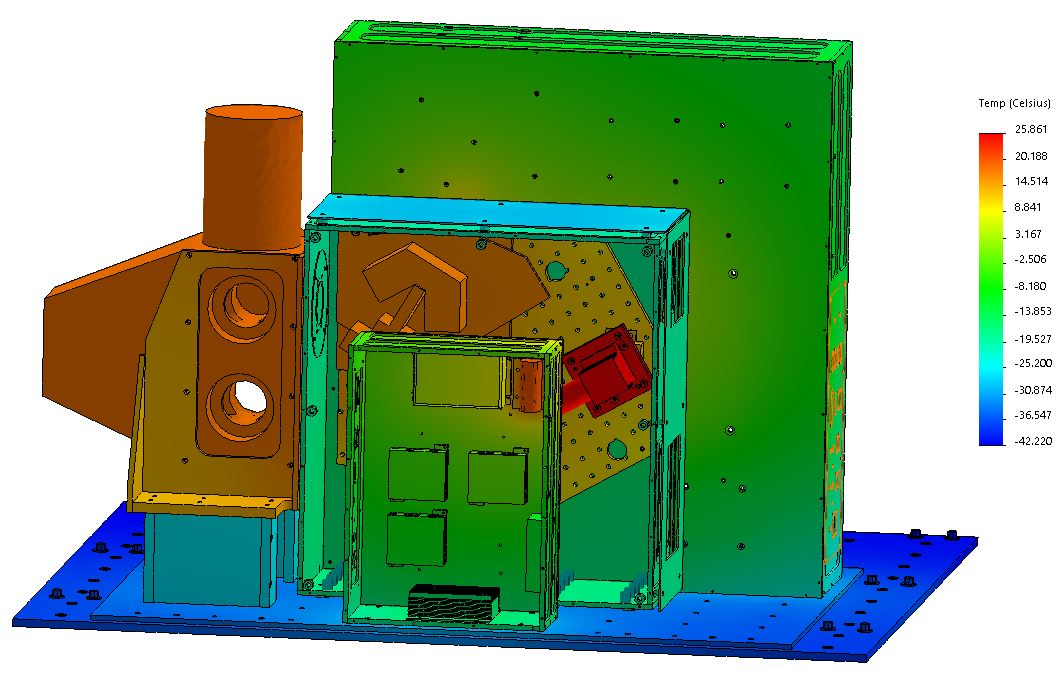
\includegraphics[width=\textwidth]{chap4_images/ascent_images/ascent_pt1/Test_30_BBEbox.JPG}
        \caption{Thermal model of LIFE instrument at the end of the ascent, Blackbody Electronics Box view.}
        \label{fig:ascent_pt2_model_bbebox}
    \end{subfigure}
    \begin{subfigure}[h]{0.9\textwidth}
        \centering
        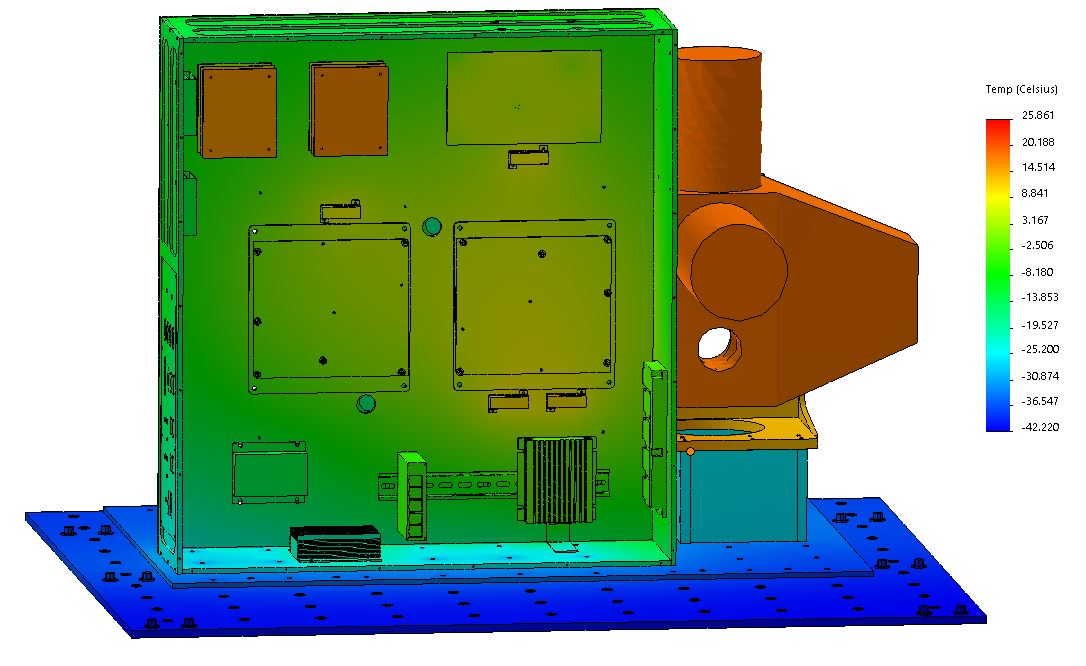
\includegraphics[width=\textwidth]{chap4_images/ascent_images/ascent_pt1/Test_30_Ebox.JPG}
        \caption{Thermal model of LIFE instrument at the end of the ascent, Electronics Box view.}
        \label{fig:ascent_pt2_model_ebox}
    \end{subfigure}
    \caption{LIFE thermal model, as the instrument is reaching the float altitude.}
    \label{ascent_pt2_model}
\end{figure}

There are too many components and loads to be able to accurately describe all values chosen and all iterations here. A list of all loads, components and plots can be automatically downloaded from SolidWorks after a simulation, and this is added as an appendix, so that all settings for the final simulation can be seen. The results from different iterations is also included in Appendix \ref{post_flight_thermal_properties_appendix}. After a total of 61 iterations, the final temperature models for the end of the first phase of the ascent and the end of the second phase of the ascent are shown in Figures \ref{ascent_pt1_model} and \ref{ascent_pt2_model}, respectively. A plot showing the simulated temperature curves of the thermal model, measured at the same locations as the on-board temperature sensors, is shown in Figure \ref{fig:ascent_temps_with_sims} as a verification of the model.

\begin{figure}
    \centering
    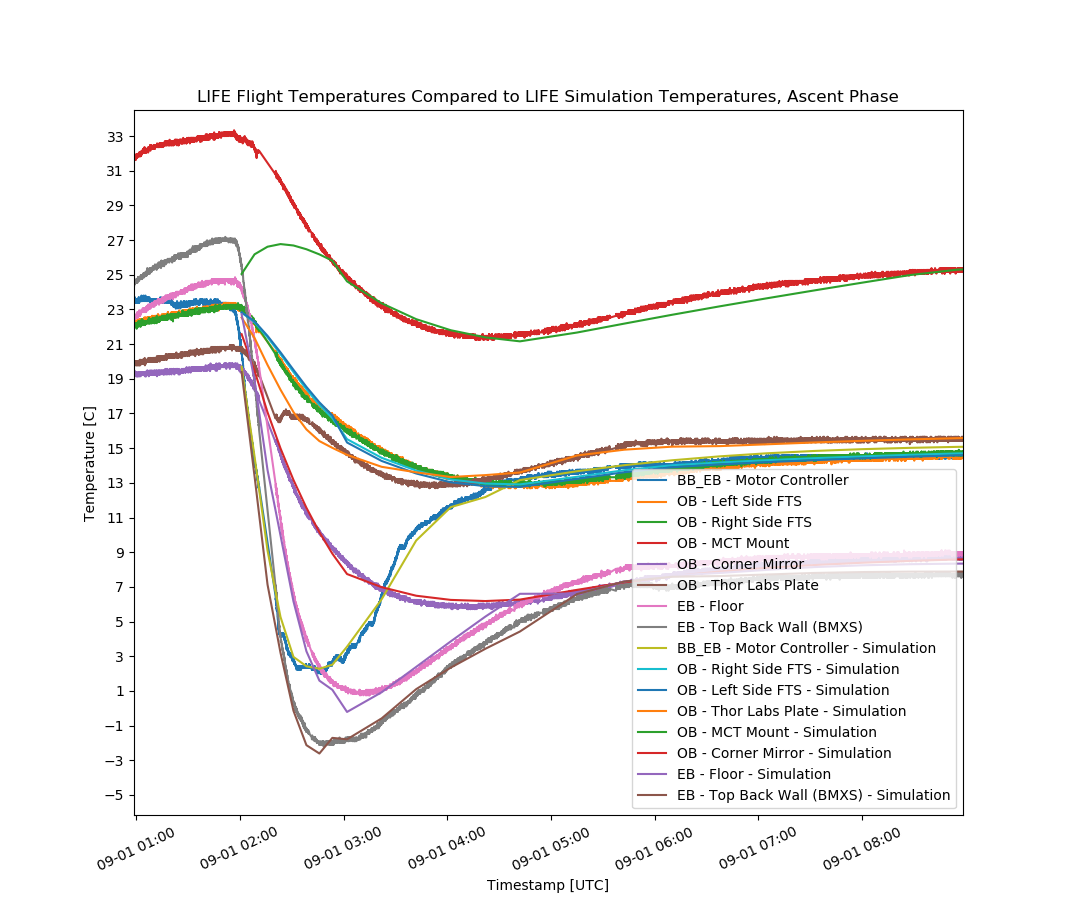
\includegraphics[width=\textwidth]{chap4_images/ascent_images/ascent_with_sim_temps_no_altitude.png}
    \caption{Flight temperatures through the ascent, compared to the simulated temperature curves after model updates.}
    \label{fig:ascent_temps_with_sims}
\end{figure}

From the plot in Figure \ref{fig:ascent_temps_with_sims}, the model now fits the ascent very well, with the largest error of 1°C. Errors in the first part of the ascent are due to the generalized initial temperatures, but they shortly begin to match the actual temperatures early in the ascent. It was ensured that the temperatures were as close as possible to the actual temperatures at the end of the simulation, so the initial temperatures of the next phase are as close as possible. The error between actual and simulated temperatures for the end of the ascent are within 0.2°C for the critical components, which is well within the goal of 1°C..

\subsection{Float}
The next phase of flight was the \textit{float} phase, or the phase where the instrument stayed steady at 36km, operated nominally and took measurements. This was the simplest part of the flight to simulate, as the environmental effects were constant throughout this stage, and convection no longer played a role. Some transient temperatures are still used for some ambient radiation temperatures, but for the most part all heat loads stay steady. This was also the part of the flight that was simulated in the TVAC chamber, and as a result no issues were expected. This stage continues until the sun rises.

\subsubsection{Measured Temperatures}
The beginning of this phase of the flight was when the ascent was officially over, and the gondola had stabilized at the required altitude. This occurred at 5:00 UTC. The sun rose just after 10:00 UTC, and began to have an affect around 10:30 UTC. When the solar flux needed to be included, the simulation was split, and that was characterized as the \textit{sunrise} phase of the flight, and is described later. The temperature measurements of the float phase, along with the gondola altitude, are shown in Figure \ref{fig:float_temps_no_sims}.

\begin{figure}
    \centering
    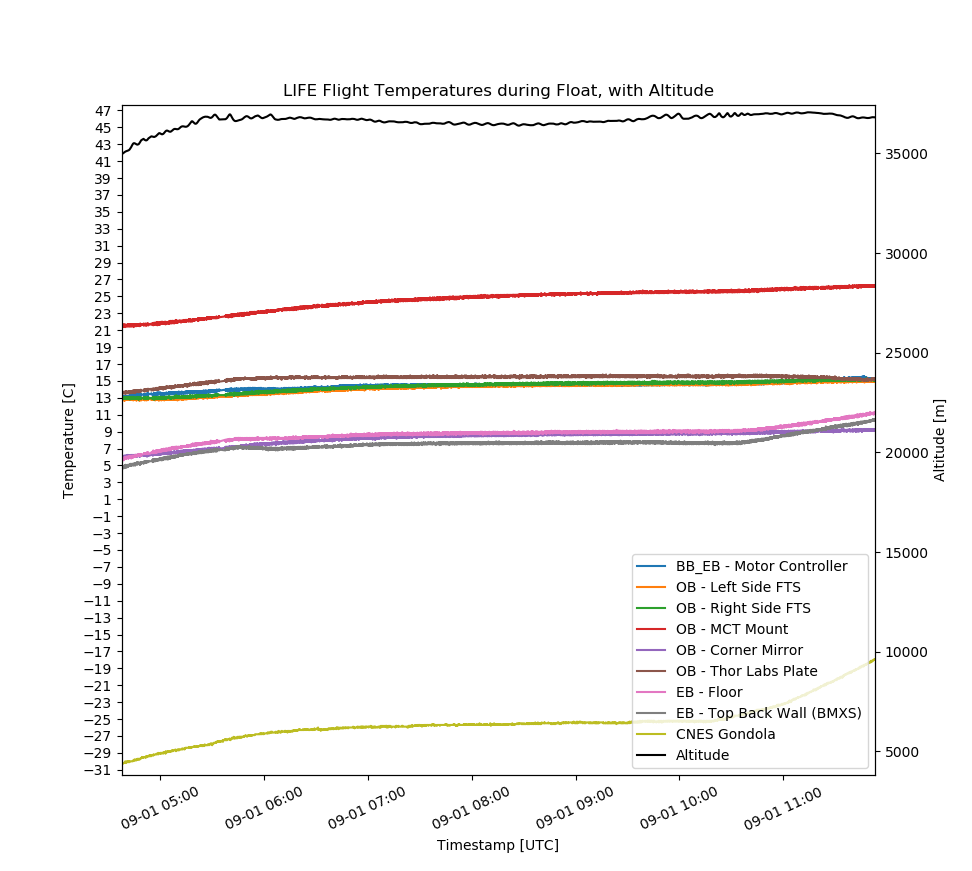
\includegraphics[width=\textwidth]{chap4_images/float_images/float_no_sim_temps.png}
    \caption{Flight temperatures through the float phase, five and a half hours where most measurements were taken.}
    \label{fig:float_temps_no_sims}
\end{figure}

The temperatures fully stabilized around 6:00 UTC. After this point, the temperatures remain very stable, until the gondola deck begins to heat at around 10:30 UTC. The warmest component was the MCT detector mount, which makes sense as the detector was dumping heat to its surroundings. All optics were kept within a couple degrees, which is ideal. The double isolation of this plate helped to keep the temperatures similar across the entire plate, which will help to remove self-emission from the resulting data. In addition, the temperature drift requirement is met; over the course of almost 6 hours, the critical optical temperatures of the corner mirror and FTS changed less than half a degree. Thus there is no problems seen in any of the Optics Box temperatures, and it ran nominally for this stage.

The Electronics Box temperatures were cooler than expected. This was due to the initial temperatures for this stage of the flight; the temperature shock of the ascent had a larger effect than was expected. Also, in comparison to the Optics Box, there is less insulation around this box and it is larger; as a result, this box would be cooled faster through both convection across the back plate and conduction in the baseplate. However, when the heaters kicked in and the instrument reached the warmer stratosphere, the temperatures steadied. Something to note was the temperature set point of the temperature controllers was higher, above 10°C. Through most of the flight, the temperatures were slightly below this. It was found that the set point of the temperature controller drifted, and as a result the amount of power sent to the heaters in the Electronics Box was lower than needed. The electronics temperature requirements were still met, but if this had happened to the temperature controller for the Optics Box, more serious issues could have occurred. A correction for this issue needs to be researched for future instruments, to ensure that temperatures are staying nominal. However, despite the temperature not being as high as planned, the heaters still managed to keep the temperatures steady, showing that power was still being applied properly. The gondola baseplate temperature of roughly -27°C was in the range of simulated tests, and is good to know for future instrument simulations.

\subsubsection{Simulation}
With only conduction and radiation to include in the simulation, and with a steadier external environment, the simulations for this phase would be simpler. A total of 17 iterations were required to produce a model accurate to what was seen during flight. This was partly due to the initial temperatures from the previous simulation, which allowed an exact starting point for this simulation, following very precise initial temperatures compared to the flight. The conductive properties for this simulation were also all kept the same from what was determined from the TVAC tests and the ascent tests.

Much of the work of the radiation was already finished as well. The view factors were determined from the ascent simulations, and to maintain continuity between the simulations could not be changed. The only other value that needed to be determined was the ambient temperature. Due to the constant temperatures of both the instrument and the environment, they could be kept the same for the entire simulation, instead of attempting to determine a time curve. This made the iterations and determining the appropriate temperatures much easier. The majority if the ambient temperatures were taken from what was seen during the flight. 

With no convection to be determined either, the only other aspect of the model that could be changed apart from the ambient temperatures was the power of the heaters. These were chosen, as with the TVAC test, from the measured instrument currents. More discussion into this is given in the full model discussion, in Section \ref{full_temp_model}. As with the ascent simulations, after a number of iterations, a thermal model was created that very closely matched the flight temperatures. Images of the final simulation are shown in Figure \ref{float_model}, and a comparison of the flight temperature curve to the simulated temperature curve is shown in Figure \ref{fig:float_temps_with_sims}.

\begin{figure}
    \centering
    \begin{subfigure}[h]{0.9\textwidth}
        \centering
        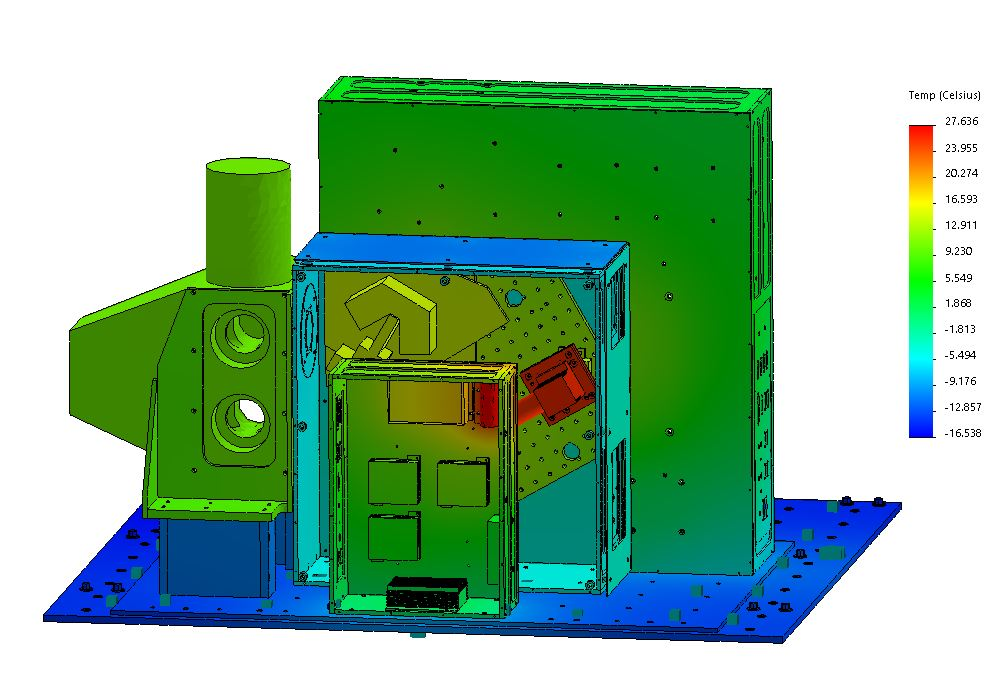
\includegraphics[width=\textwidth]{chap4_images/float_images/Test_16_BBEbox.JPG}
        \caption{Thermal model of LIFE instrument at the end of the float phase, Blackbody Electronics Box view.}
        \label{fig:float_model_ebox}
    \end{subfigure}
    \begin{subfigure}[h]{0.9\textwidth}
        \centering
        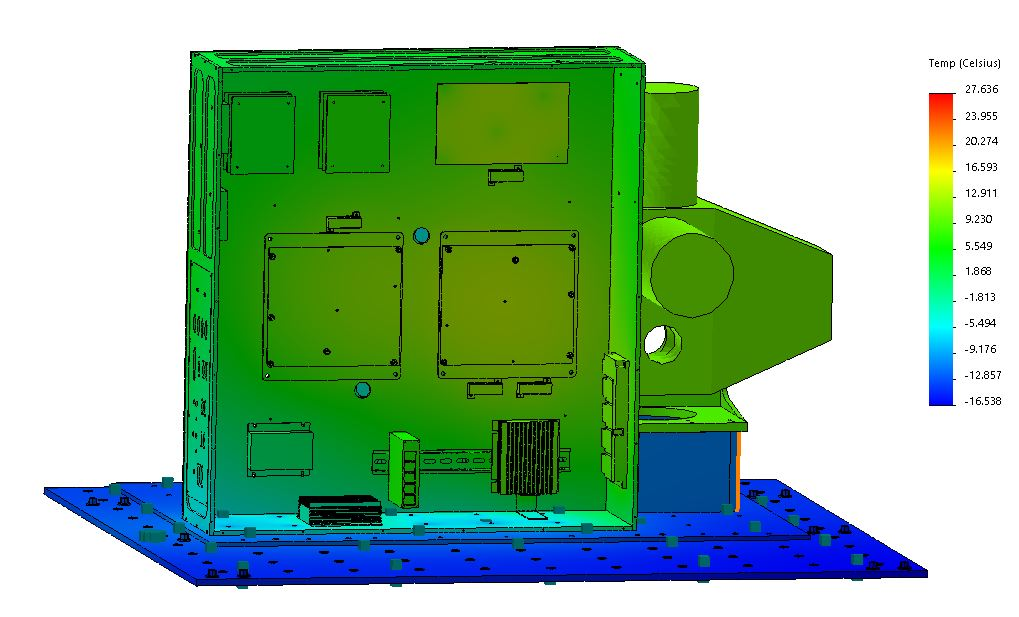
\includegraphics[width=\textwidth]{chap4_images/float_images/Test_16_Ebox.JPG}
        \caption{Thermal model of LIFE instrument at the end of the float phase, Electronics Box view.}
        \label{float_model_ebox}
    \end{subfigure}
    \caption{LIFE thermal model at the end of the nominal float stage of the flight.}
    \label{float_model}
\end{figure}

\begin{figure}
    \centering
    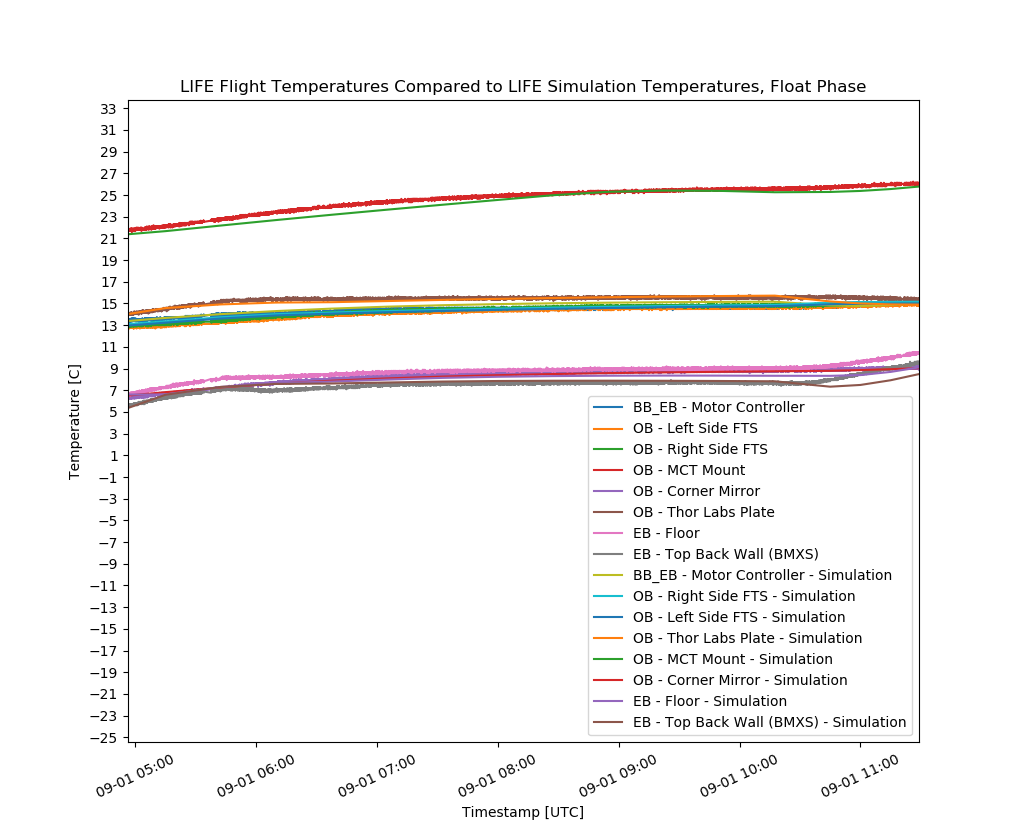
\includegraphics[width=\textwidth]{chap4_images/float_images/float_with_sim_temps.png}
    \caption{Flight temperatures during the float phase, compared to the simulated temperature curves after model updates.}
    \label{fig:float_temps_with_sims}
\end{figure}

In Figure \ref{fig:float_temps_with_sims} the model now matches the actual temperatures very well. All temperatures match with an maximum error of 1°C, and the error on critical components less than 0.2°C. Once again, the final temperatures of this stage were very carefully simulated to match the actual temperatures as closely as possible, so the initial temperatures of the sunrise simulation match as closely as possible. Thermal loads for this simulation as well as the iterated thermal values can be found in the appendix.

\subsection{Sunrise}
The final part of the flight, known as the \textit{sunrise} stage, took place from 10:30 UTC to the instrument was turned off prior to the descent, at 14:30 UTC. As mentioned previously this stage was never expected to occur, however there was difficulty in finding a landing zone for the gondola and the descent was delayed. While the instrument was originally planned to be turned off, it was decided that this was an opportunity to see how the model operated thermally in the sunlight. As there was time to create the thermal model for the sunlight and data was saved, this could be added to the entire atmospheric instrument thermal model.

\subsubsection{Measured Temperatures}
This stage of flight began as soon as temperatures began to increase after sunrise. They steadily rose throughout the remainder of the flight. While temperatures would be expected to begin levelling out again at some point, it is not surprising that the temperatures increased so quickly. The sun at high altitudes has a dramatic thermal effect, and no fans in the instrument were operating. There were also no vents anywhere either, as these were all enclosed to prevent any damage or intake to the inside of the boxes during the ascent. As a result the electronics steadily increased in temperature until they began to reach maximum allowable temperatures, and the instrument was turned off. A plot of these temperatures for this stage is shown in Figure \ref{full_temp_model}.

\begin{figure}
    \centering
    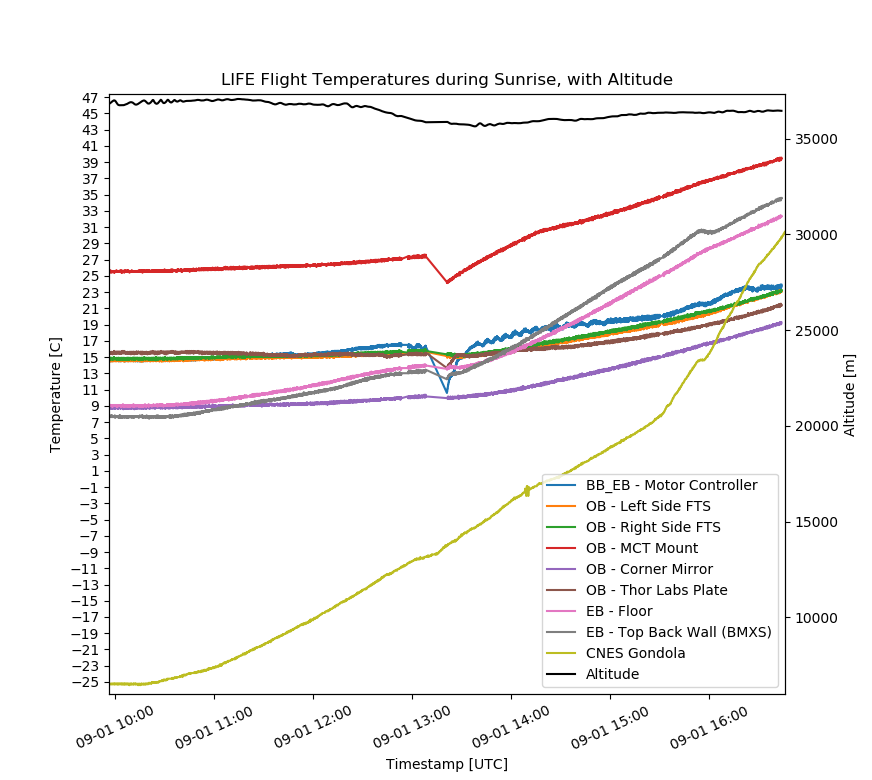
\includegraphics[width=\textwidth]{chap4_images/sunrise_images/sunrise_no_sim_temps.png}
    \caption{Flight temperatures as the sun rose and shone on the instrument, up until the end of the flight.}
    \label{fig:sunrise_temps_no_sims}
\end{figure}

The first plot of the figure to point out is the drop around 13:00 UTC. This was due to an initial shutoff of the instrument, when the descent was expected to begin. When it was determined that the flight would continue for at least another hour after, the instrument was turned back on to take more measurements as well as to gather temperature measurements. However this drop does show the effect of turning off the electronics, and the amount of power that they generate. Most temperatures dropped by at least 2°C in just a few minutes of no power. When power was restored the temperatures increased again quickly. 

As with the previous stages of the flight, there is a large difference in behaviour between the electronics boxes and the Optics Box. With the sun shining directly on the rear plate of the Electronics Box, temperatures climbed very quickly in the last few hours of flight. However, even with the same sun shining on the Optics Box, the temperatures remained very steady until the last few hours. This shows that the outer radiation plate was operating as expected; while the outer plate was absorbing the flux of the sun, very little of that heat was being transferred to the inner box, and then to the optics. Only after the outer box was heated for a considerable amount of time did the effect of sun begin to show on the interior components. This shows that if the instrument was expected to operate in daylight, the addition of similar radiation plates to sensitive areas of other boxes (the top of the Electronics Box for example, where the temperature-sensitive BMXS board is mounted) would allow the instrument to be used without issue. In addition it is noted that for most daylight flights extra shielding is used over the gondola to mitigate sun-exposure. This may have helped maintain the LIFE temperatures to their required range even with no other changes to the instrument. Finally, the temperature of the gondola baseplate is noted; this shows how quickly the temperature of the gondola itself rose, and that the rise in temperature of LIFE was expected.

\subsubsection{Simulation}
For complexity, this simulation is between the difficulties of the previous two simulations. It does not have the quick changes in temperature and environment of the ascent, nor does it have convection. However the environment is not nearly as steady as the float portion of the flight. Most importantly, the effect of the sun must be included in this simulation. As with the float, the conductive properties and initial temperatures are already well known. The main properties that must be iterated through for the final stage is the solar flux effect and the ambient temperature of the radiation.

The heat flux from the sun was more difficult to simulate than expected. The solar flux from the sun is well known in orbit to be 1400 $W/m^2$. However, this heat flux decreases through the atmosphere, as some of this flux is absorbed by atmospheric molecules. Like convection in the atmosphere, there is no literature to explain what solar flux is to be expected at what altitude. Beyond this, the sun was not shining directly on the instrument for the entire stage of the flight, nor with its full intensity. Only part of the sun could sometimes be seen, or sometimes it may have been shining on the side of the gondola. Unfortunately adding the solar flux was not as easy as adding a 1400 $W/m^2$ heat load to the side of the instrument. Through simulation iterations, it was eventually determined that a somewhat exponential curve of flux led to the desired temperatures. Starting at 0 $W/m^2$ for the beginning of the phase, it increased to 800 $W/m^2$. It is believed that the sun did not shine directly on the instrument, and was warmed either through the wall of the gondola or through reflections. More data on the effect of sunlight is needed to verify this.

The final changes were made for the radiation ambient temperatures. It was similar to the previous simulations, which was changing the ambient temperatures to what was seen from the flight data. In addition to this however, the ambient temperature was increased for the outer parts of the instrument that may have been warmed by the sun or from parts of the gondola which were warmed. The ambient temperature of radiation for the top of the boxes as well as the sides was chosen to increase to upwards of 30°C by the end of the flight.

\begin{figure}
    \centering
    \begin{subfigure}[h]{0.8\textwidth}
        \centering
        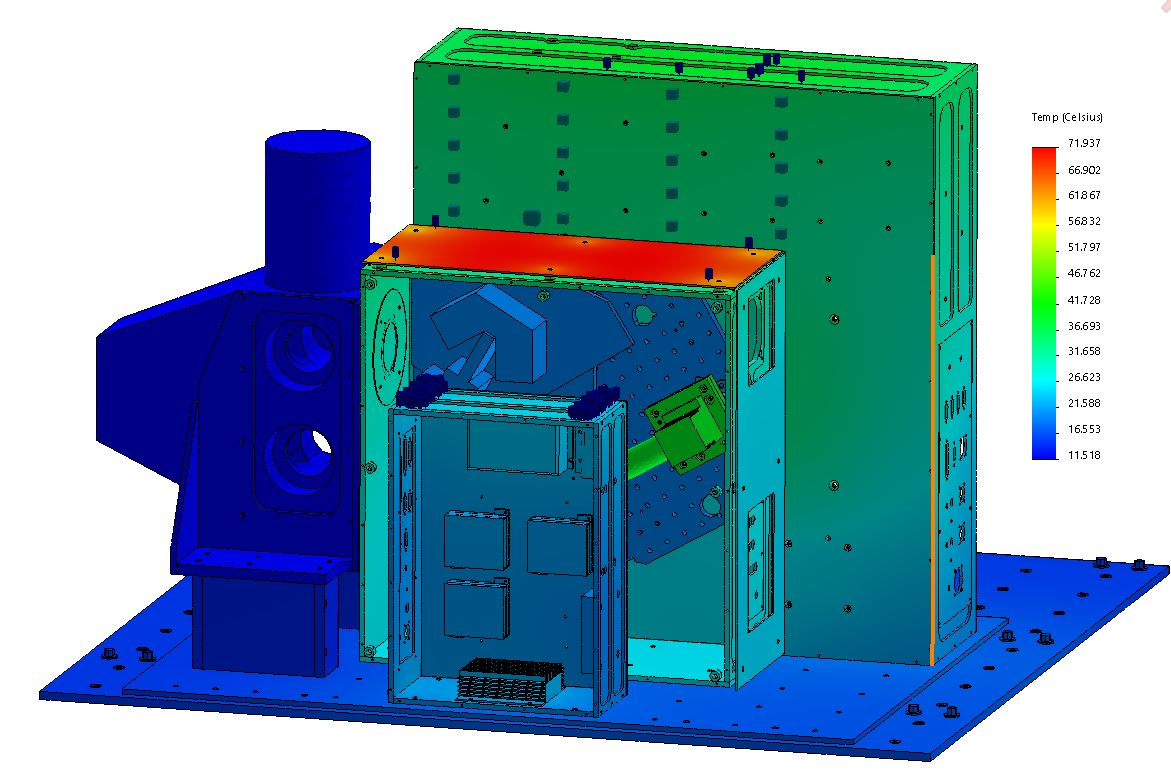
\includegraphics[width=\textwidth]{chap4_images/sunrise_images/Test_11_BBEbox.JPG}
        \caption{Thermal model of LIFE instrument at the end of the entire flight, Blackbody Electronics view.}
        \label{fig:sunrise_model_ebox}
    \end{subfigure}
    \begin{subfigure}[h]{0.9\textwidth}
        \centering
        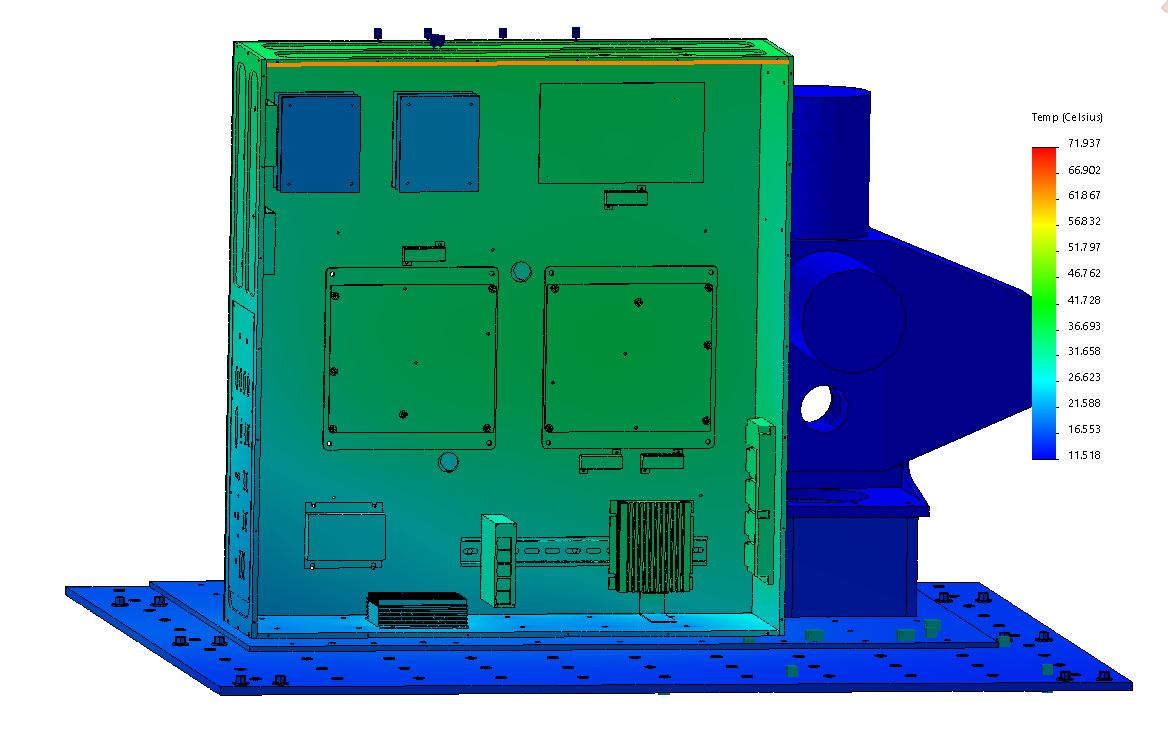
\includegraphics[width=\textwidth]{chap4_images/sunrise_images/Test_11_Ebox.JPG}
        \caption{Thermal model of LIFE instrument at the end of the entire flight, Electronics Box view.}
        \label{sunrise_model_ebox}
    \end{subfigure}
    \caption{LIFE thermal model at the end of the sunrise stage of the flight, shortly before descent.}
    \label{sunrise_model}
\end{figure}

\begin{figure}
    \centering
    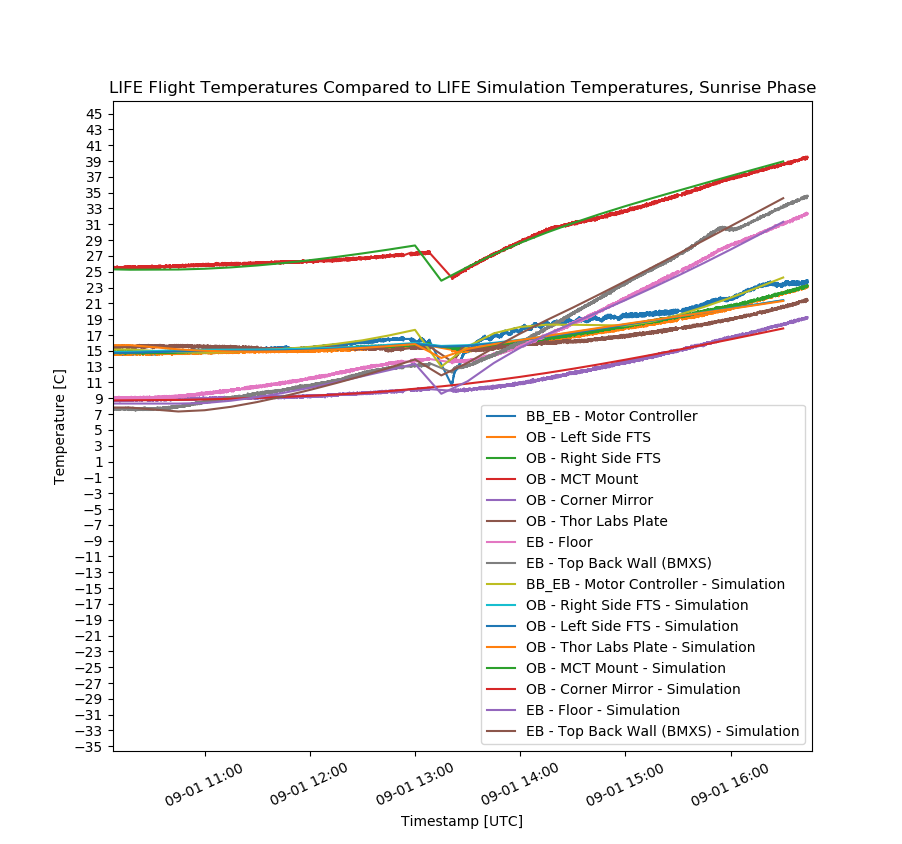
\includegraphics[width=\textwidth]{chap4_images/sunrise_images/sunrise_with_sim_temps.png}
    \caption{Flight temperatures during the sunrise phase, compared to the simulated temperature curves after model updates.}
    \label{fig:sunrise_temps_with_sims}
\end{figure}

After 16 iterations a satisfactory thermal model for this stage was created. Images of this model are shown in Figure \ref{sunrise_model}, and the comparison of the simulated temperatures to the actual temperatures is shown in Figure \ref{fig:sunrise_temps_with_sims}. A interesting note from the thermal simulations, the effect of the solar heating on the top of the Optics Box is very obvious, heating the top plate to upwards of 70°C. The rest of the box still maintains a much cooler overall temperature.

Overall the model simulations the sunrise well. There is some error around the shutoff of the instrument, and this is due to the time step of the simulation. The power off time is roughly 10 minutes, and the entire phase of the flight is four hours. It would take a very long time to be able to run the simulation with steps of 10 minutes, so a coarser step is chosen. As a result the power off time in the simulation is slightly longer than the actual time. However, the temperatures still match in this region reasonably well. The temperatures are within 1°C of the actual temperatures, and as such the model is deemed successful. As before, more information about the thermal loads and temperature values can be found in the appendix.

\subsection{Full model}\label{full_temp_model}
With all sections done separately, they can be brought together as one full model. A comparison of the actual and simulated temperature curves for the entire flight is shown in Figure \ref{fig:full_flight_temps_with_sim}. The simulated temperatures overall now match very well with what was seen during flight. However, all thermal loads used still need to be verified with a thermal model of another instrument, and some thermal loads may need to be tweaked over what was used here. Still, this provides a starting point for future thermal simulations.

\begin{figure}
    \centering
    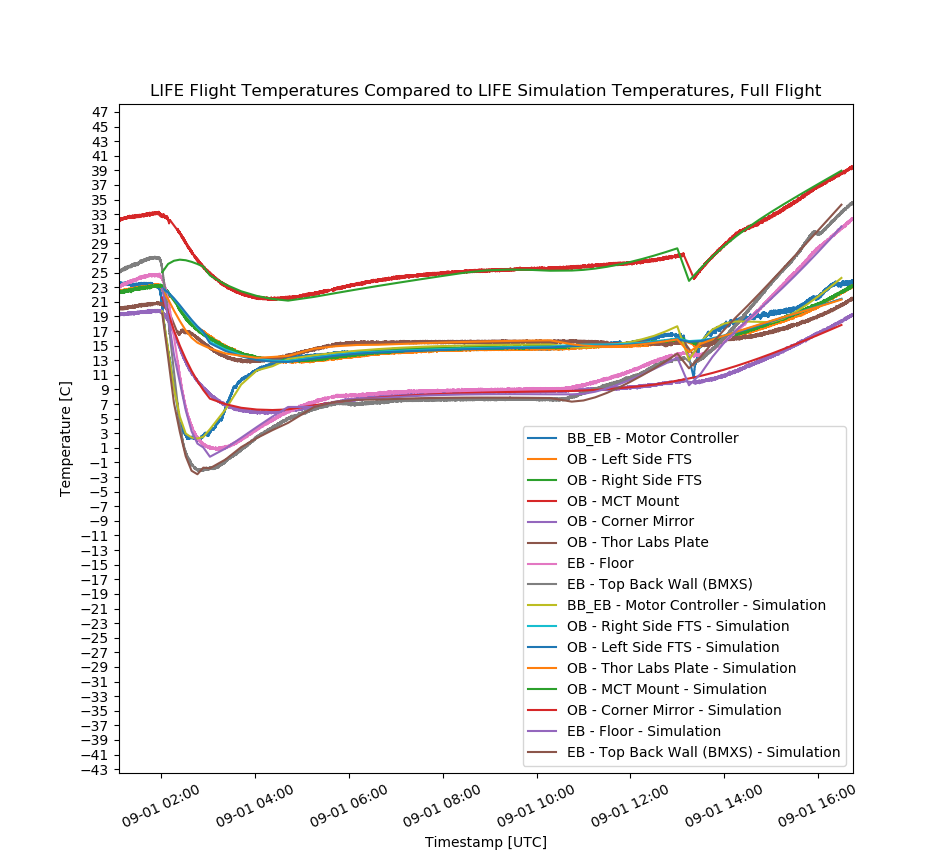
\includegraphics[width=\textwidth]{chap4_images/full_flight_with_sim_temps.png}
    \caption{The actual and simulated temperature curves for the entire flight.}
    \label{fig:full_flight_temps_with_sim}
\end{figure}

Another way that this model can be verified is by comparing the heater currents used in the simulation to what was seen during the flight. The power sent to the heaters was tweaked in the simulation to help match the flight temperatures, but it must be ensured that the power curves that were used still match the measured current during flight. A current curve for the Optics Box/Electronics Box heaters and a current curve for the Blackbody box heater is shown in Figure \ref{fig:actual_sim_current}.

\begin{figure}
    \centering
    \begin{subfigure}[h]{0.8\textwidth}
        \centering
        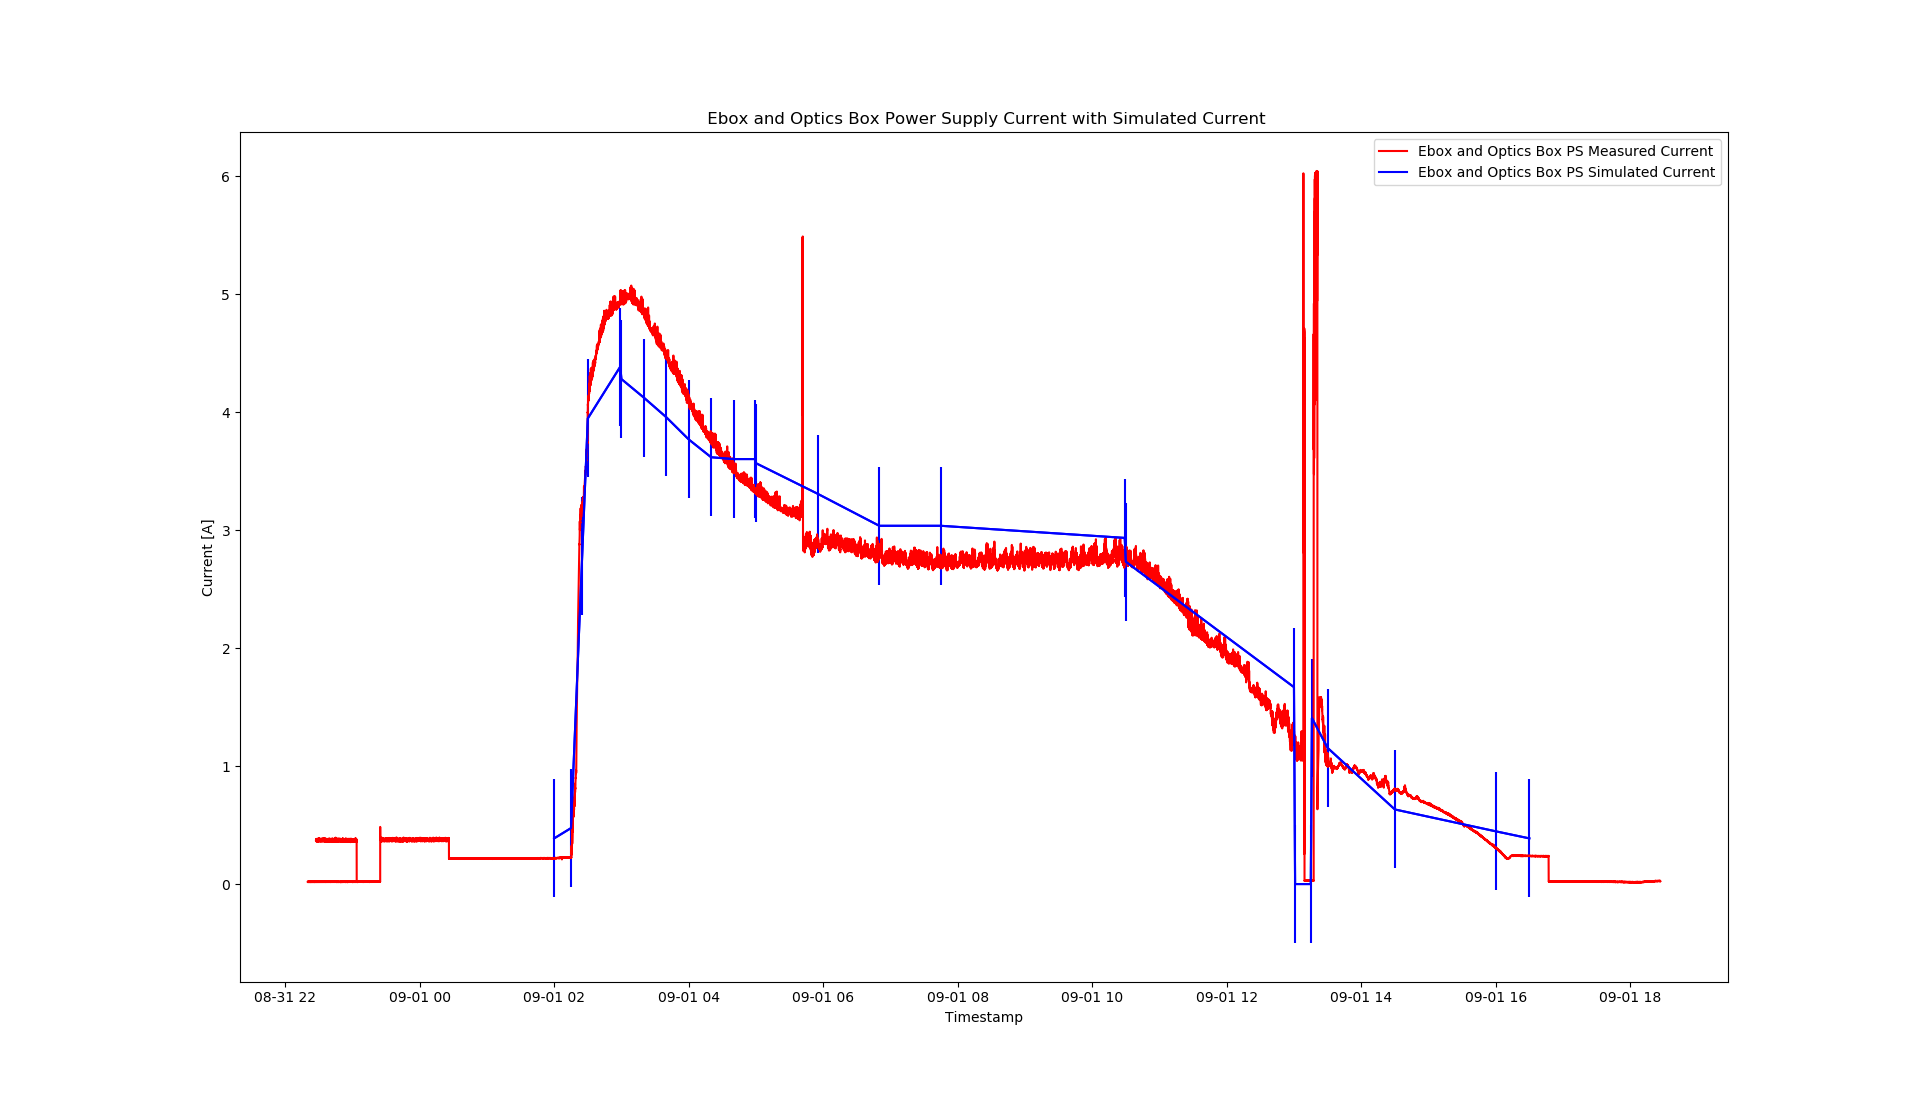
\includegraphics[width=\textwidth]{chap4_images/Ebox_OBox_I_sim_and_actual.png}
        \caption{Actual and simulated current for the Optics Box and Electronics Box heater current.}
        \label{fig:actual_sim_current_obox_ebox}
    \end{subfigure}
    \begin{subfigure}[h]{0.9\textwidth}
        \centering
        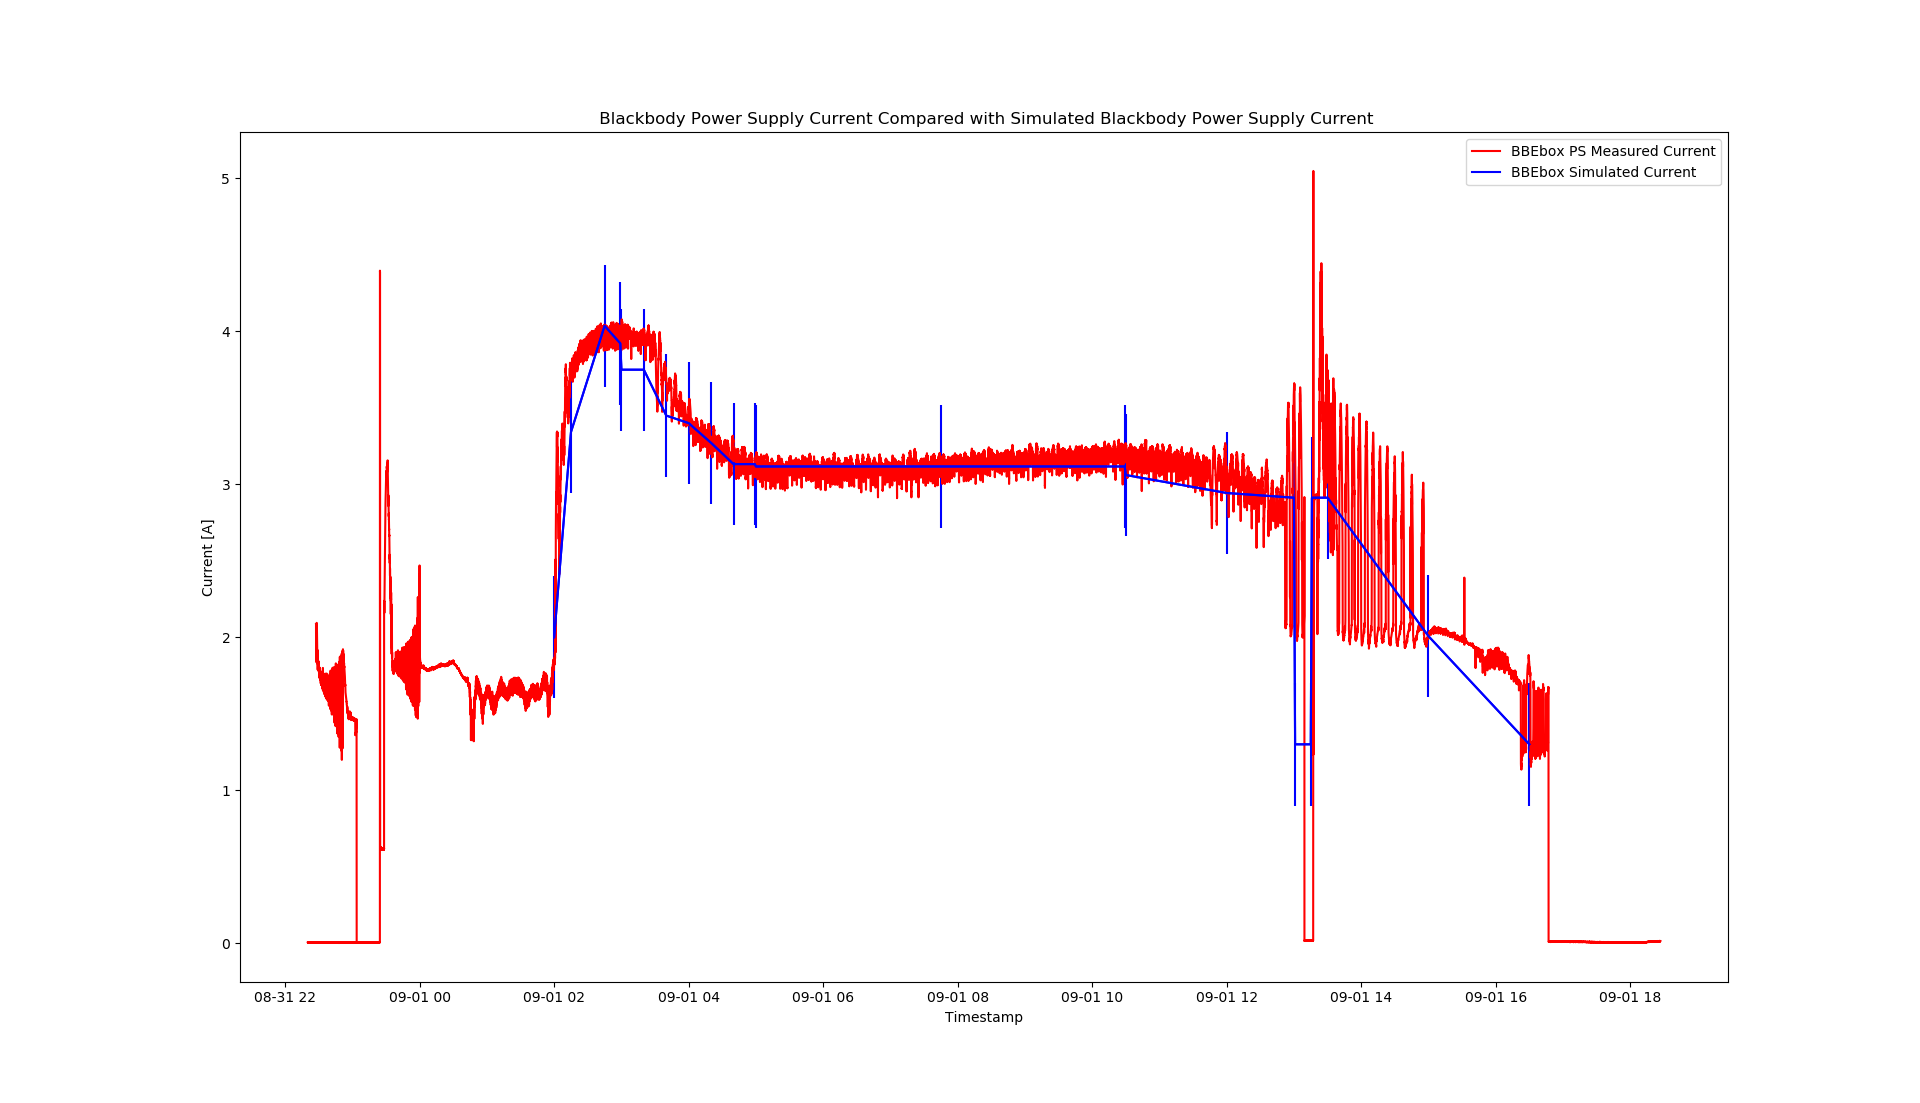
\includegraphics[width=\textwidth]{chap4_images/BBEbox_I_sim_and_actual.png}
        \caption{Actual and simulated current for the Blackbody Electronics Box heater current.}
        \label{fig:actual_sim_current_bbebox}
    \end{subfigure}
    \caption{A comparison between the current curves of what was measured during flight, and what was input into the simulation.}
    \label{fig:actual_sim_current}
\end{figure}

A margin of error is required for each system, for different reasons. In the Blackbody Electronics Box, this is to take into account that the measured current is also being used to power the blackbody system, not just the heater. This is known to be roughly 1.2A, however it can vary depending on the external environment temperatures, but it could not be measured directly. An error is included of 0.5A, to take into account the oscillation that could occur from the operation of the blackbody system. With the other boxes, the heater power is also running a few smaller systems, which is not directly taken into account by the simulations, with a current of 0.3A. As with the blackbody system power, these could oscillate, so the error is included to account for this.

Overall, the simulated temperature curve matches, within error, what was measured during flight. The overall shape is expected, with most of the power needed at the beginning to counteract the steep drop in temperatures through the ascent, leveling out around the float, and slowly turning off as the sun begins to heat the instrument. With this helping to verify the thermal model, there is more confidence that the thermal values chosen in the simulation accurately model high-altitude atmospheric conditions. This model can be used as a baseline in other thermal models of similar atmospheric instruments, which will help to gain confidence in future models and ensure those instruments will survive the flight environment.

\section{Summary}
In this chapter, all post-flight progress was discussed. The campaign and the overall results of the flight were discussed first. The flight was a success, with all thermal requirements being met, and the instrument operating nominally. Many measurements were taken over the course of the 14 hour flight, and temperature data measured that could be used to help verify the thermal model. The mechanical results were also discussed, with the instrument surviving the harsh landing well but with some damage. The damage reviewed, and next steps for the instrument are being determined.

The main aspect of this chapter was the creation and discussion of the flight temperature model. With the temperatures well simulated for a survival test of the float portion of the flight, a more detailed model of the entire flight would be created. The temperatures measured were used to create a thermal model of all stages of flight that would match the temperatures seen at all phases, of ascent, float, and sunrise. Each of these phases were created and simulated in turn in SolidWorks, using some data from the flight and some known information about the flight environment. However, there is very little research on some of the more specific thermal properties of the atmosphere, such as convection. This model was built to gain some insight on these properties, by iterating through estimations of these properties until the simulation matched the flight. It is hoped that in the future this model can be used for other atmospheric instrument flights and the model can be improved through more flight data.

